%%%%%%%%%%%%%%%%%%%%%%%%%%%%%%%%%%%%%%%%
%%%%%%%%%%%%%%%%%%%%%%%%%%%%%%%%%%%%%%%%
\beginsupplement
%%%%%%%%%%%%%%%%%%%%%%%%%%%%%%%%%%%%%%%%
%%%%%%%%%%%%%%%%%%%%%%%%%%%%%%%%%%%%%%%%

\section{Supplementary Figures}

\begin{figure}[!h]
    %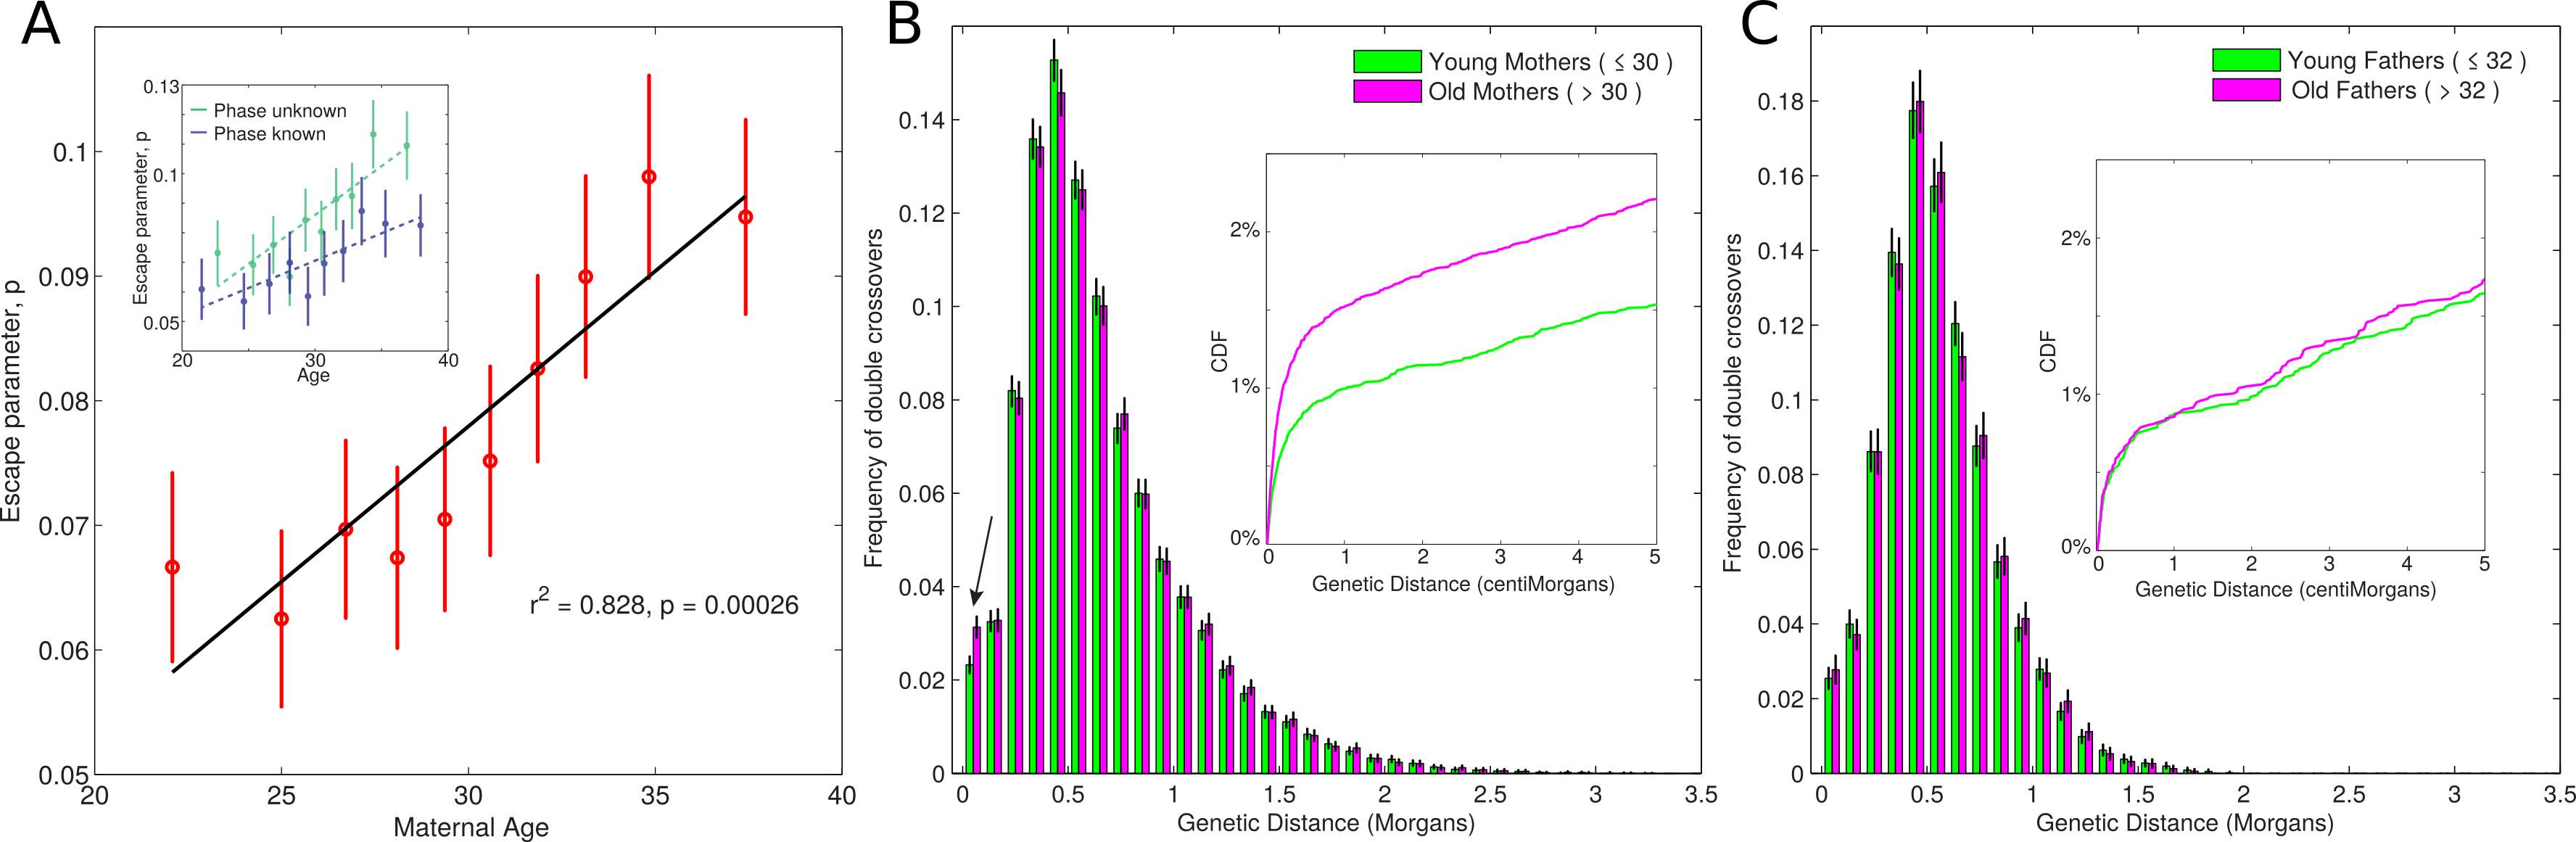
\includegraphics[width=\textwidth]{cointEscape/figs/Figure4.png}
    %\vspace{-20pt}
    \captionTitle{\textbf{Age distributions within the filtered dataset.}}{
        The left hand panel shows the distribution for phase-unknown individuals, where the parental ages were averaged across children. 
        The right hand panel shows data for the phase-known meioses where the parental age at the time of childbirth is known.
        Lines indicate the mean of each distribution. 
        Note that some families were excluded from analysis by 23andMe on the basis age to protect privacy, as seen from the truncated distribution of maternal ages in the right hand panel.  
       \label{fig:cointFS1}}
\end{figure}

\begin{figure}[!h]
    %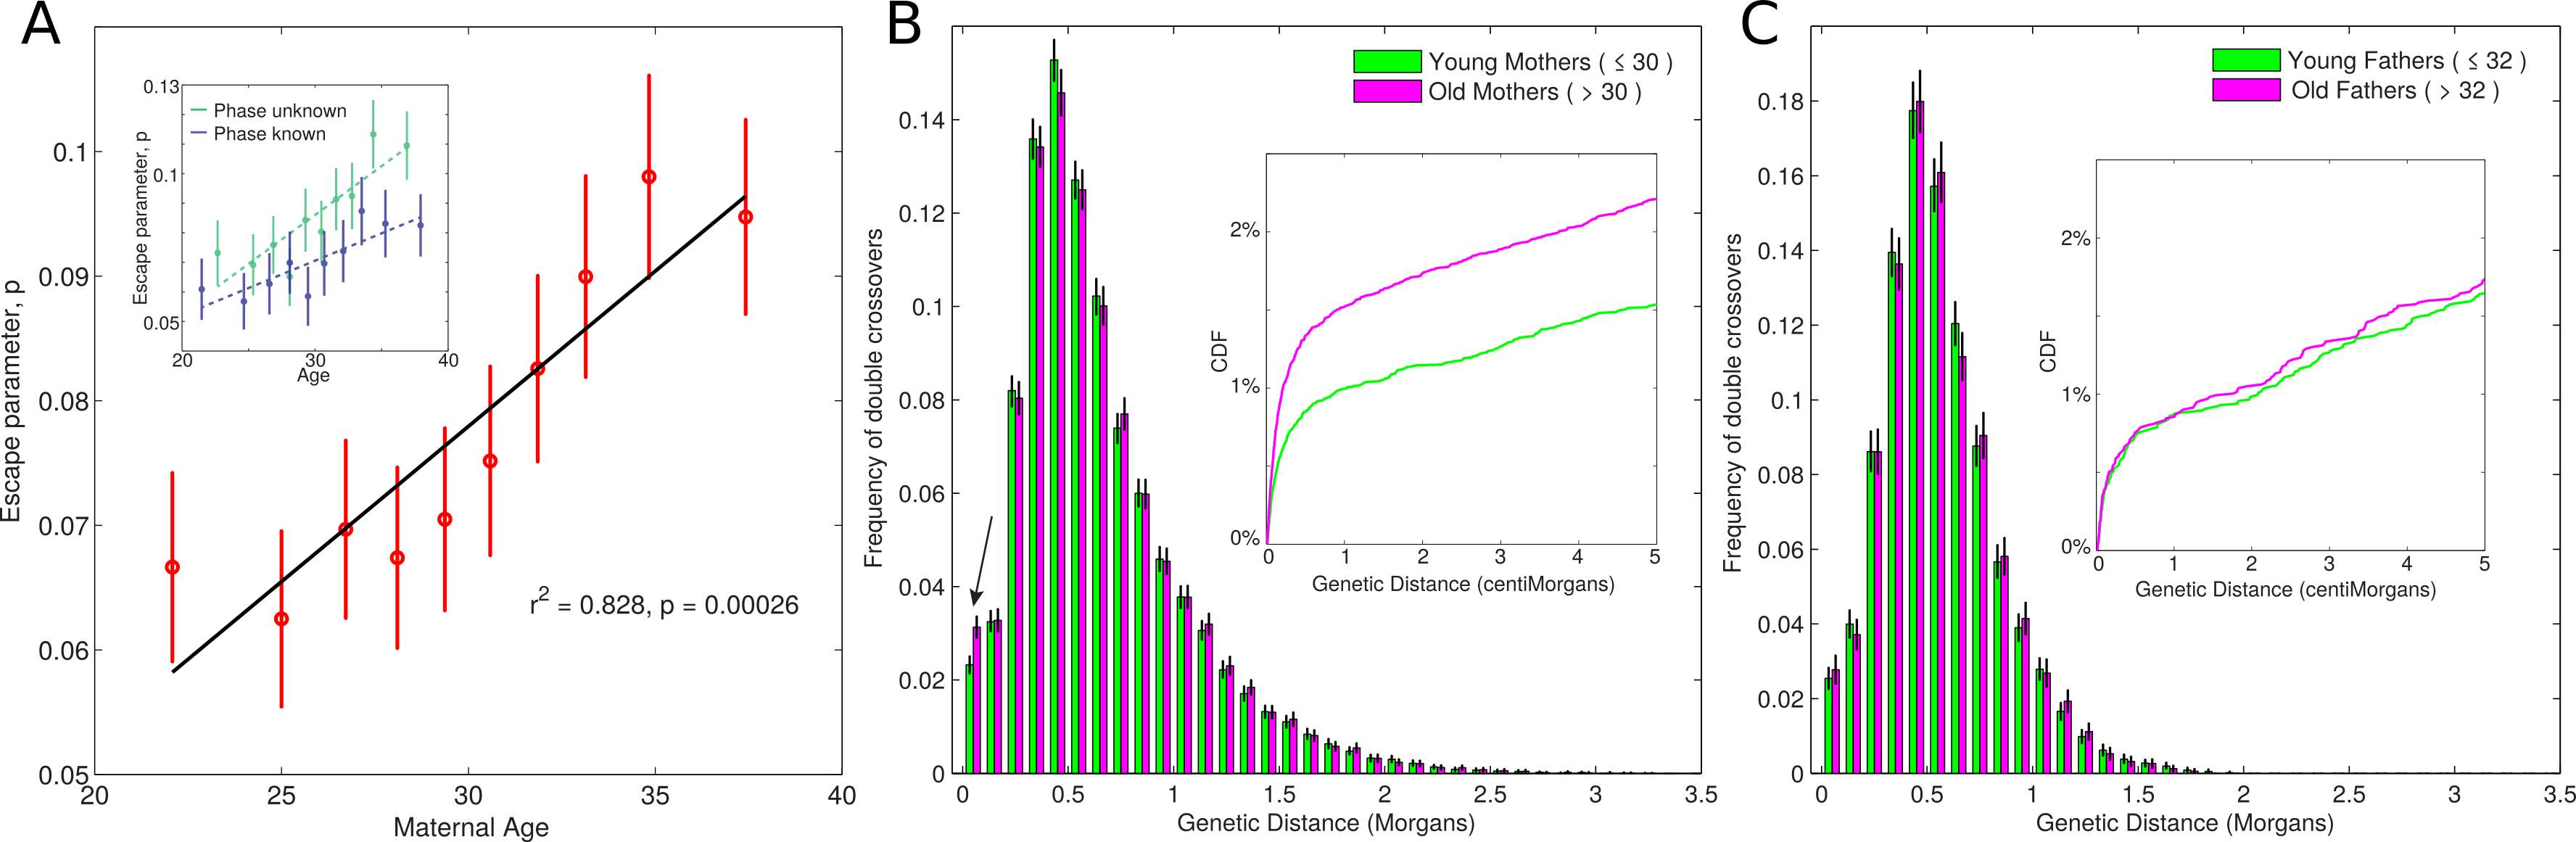
\includegraphics[width=\textwidth]{cointEscape/figs/Figure4.png}
    %\vspace{-20pt}
    \captionTitle{\textbf{Data grooming.}}{
        A) Chromosome 10 map before filtering.
        Genetic maps from the 23andMe data are shown in bold lines, whereas the genetic maps from deCODE are shown as thin lines.
        Separate maps are shown for females(red), males (blue), and sex-averaged (black). 
        Also shown are regions highlighted in grey that represent gaps in the reference assembly, the largest of which being the centromere at around 40Mb.
        B) Clustering of recombination events occurring within 1 Mb of each other within single individuals.
        Each plot shows the number of events within 1 Mb of each other on a log$_{10}$ scale as a function of physical position on each chromosome.
        A large number of these event pairs can be observed on chromosome 10, although other large peaks can also be observed on, for example, chromosomes 8 and 15.
        The dashed line represents the 99.9\% percentile of the distribution, and was used as a threshold for filtering.
        C) Chromosome 10 map after filtering.   
       \label{fig:cointFS2}}
\end{figure}

\begin{figure}[!h]
    %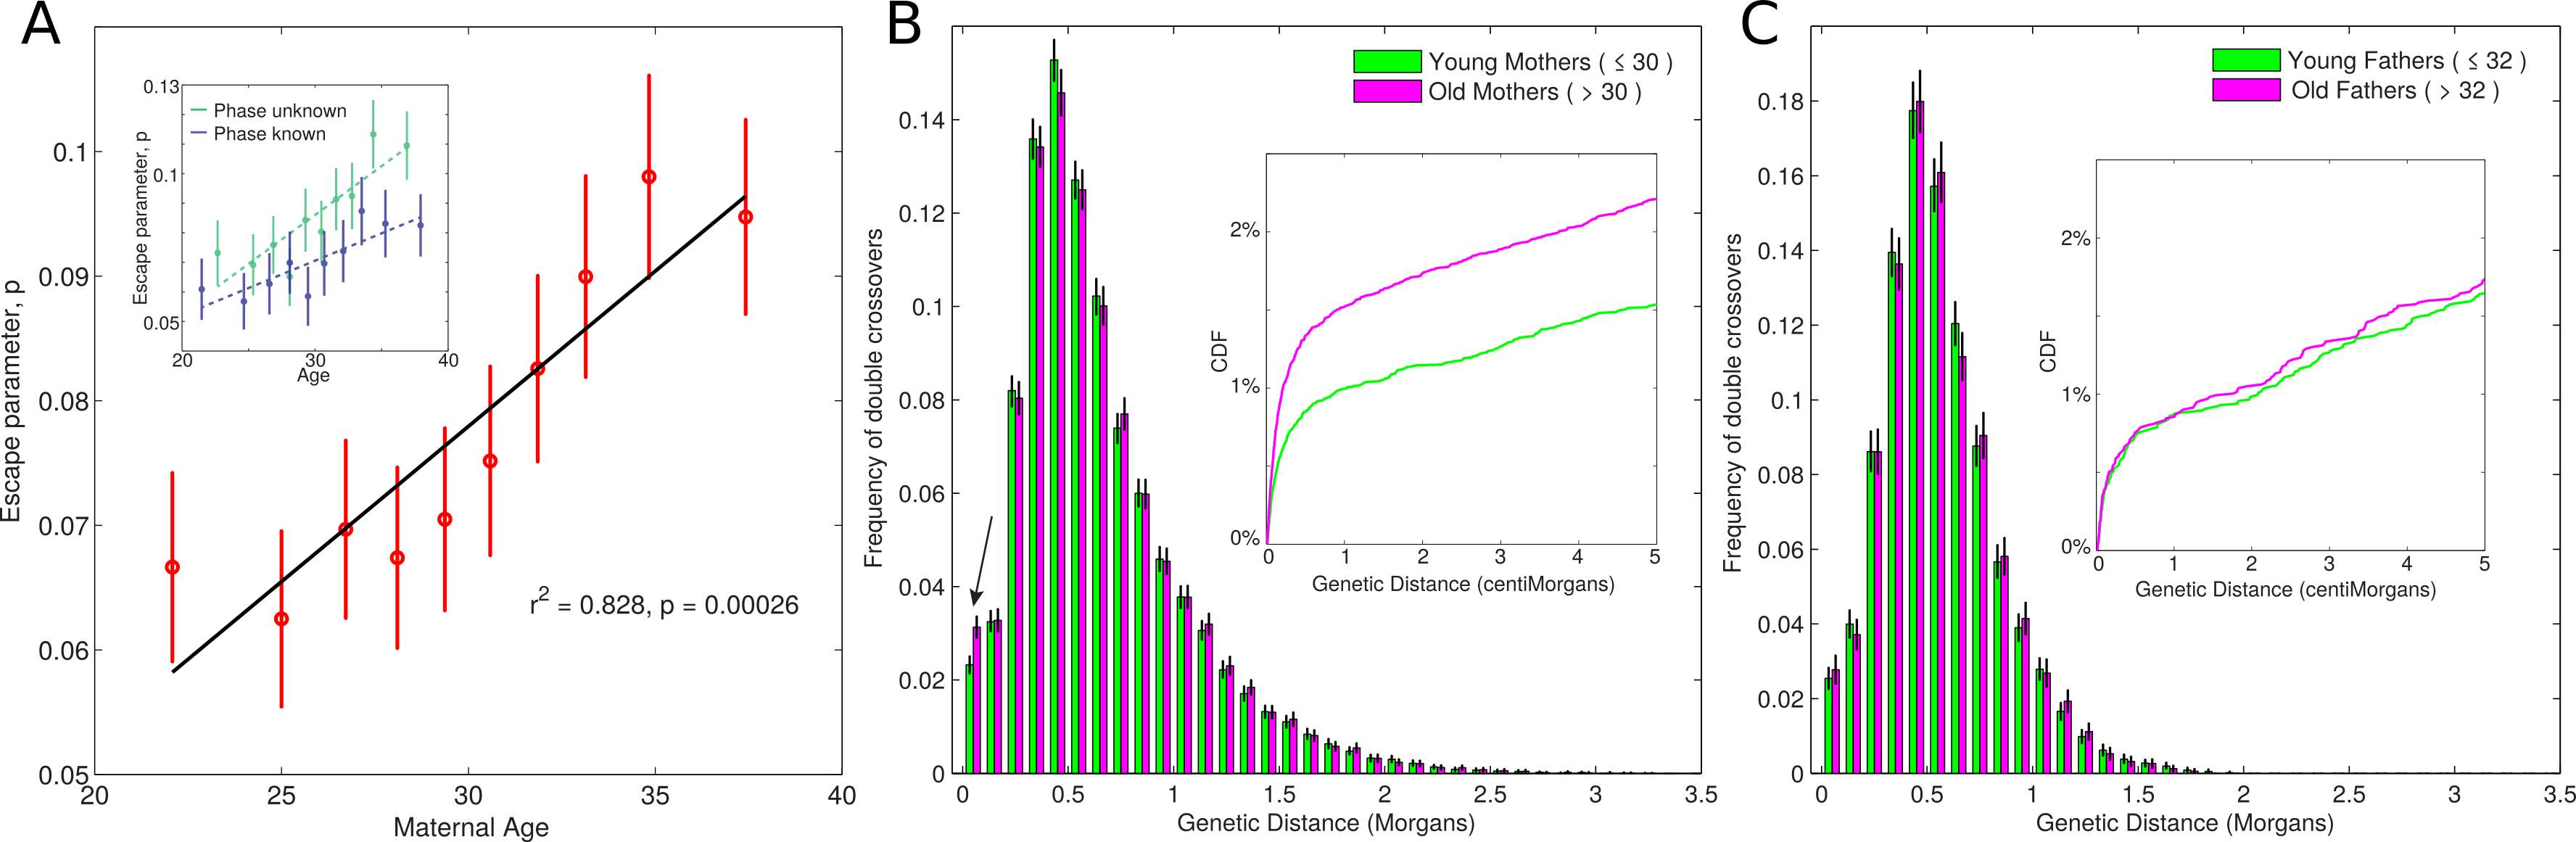
\includegraphics[width=\textwidth]{cointEscape/figs/Figure4.png}
    %\vspace{-20pt}
    \captionTitle{\textbf{Empirical cumulative distance function of crossover localization distances.}} { 
        Red labels indicate the interval distances at the distribution deciles.  
       \label{fig:cointFS3}}
\end{figure}

\begin{figure}[!h]
    %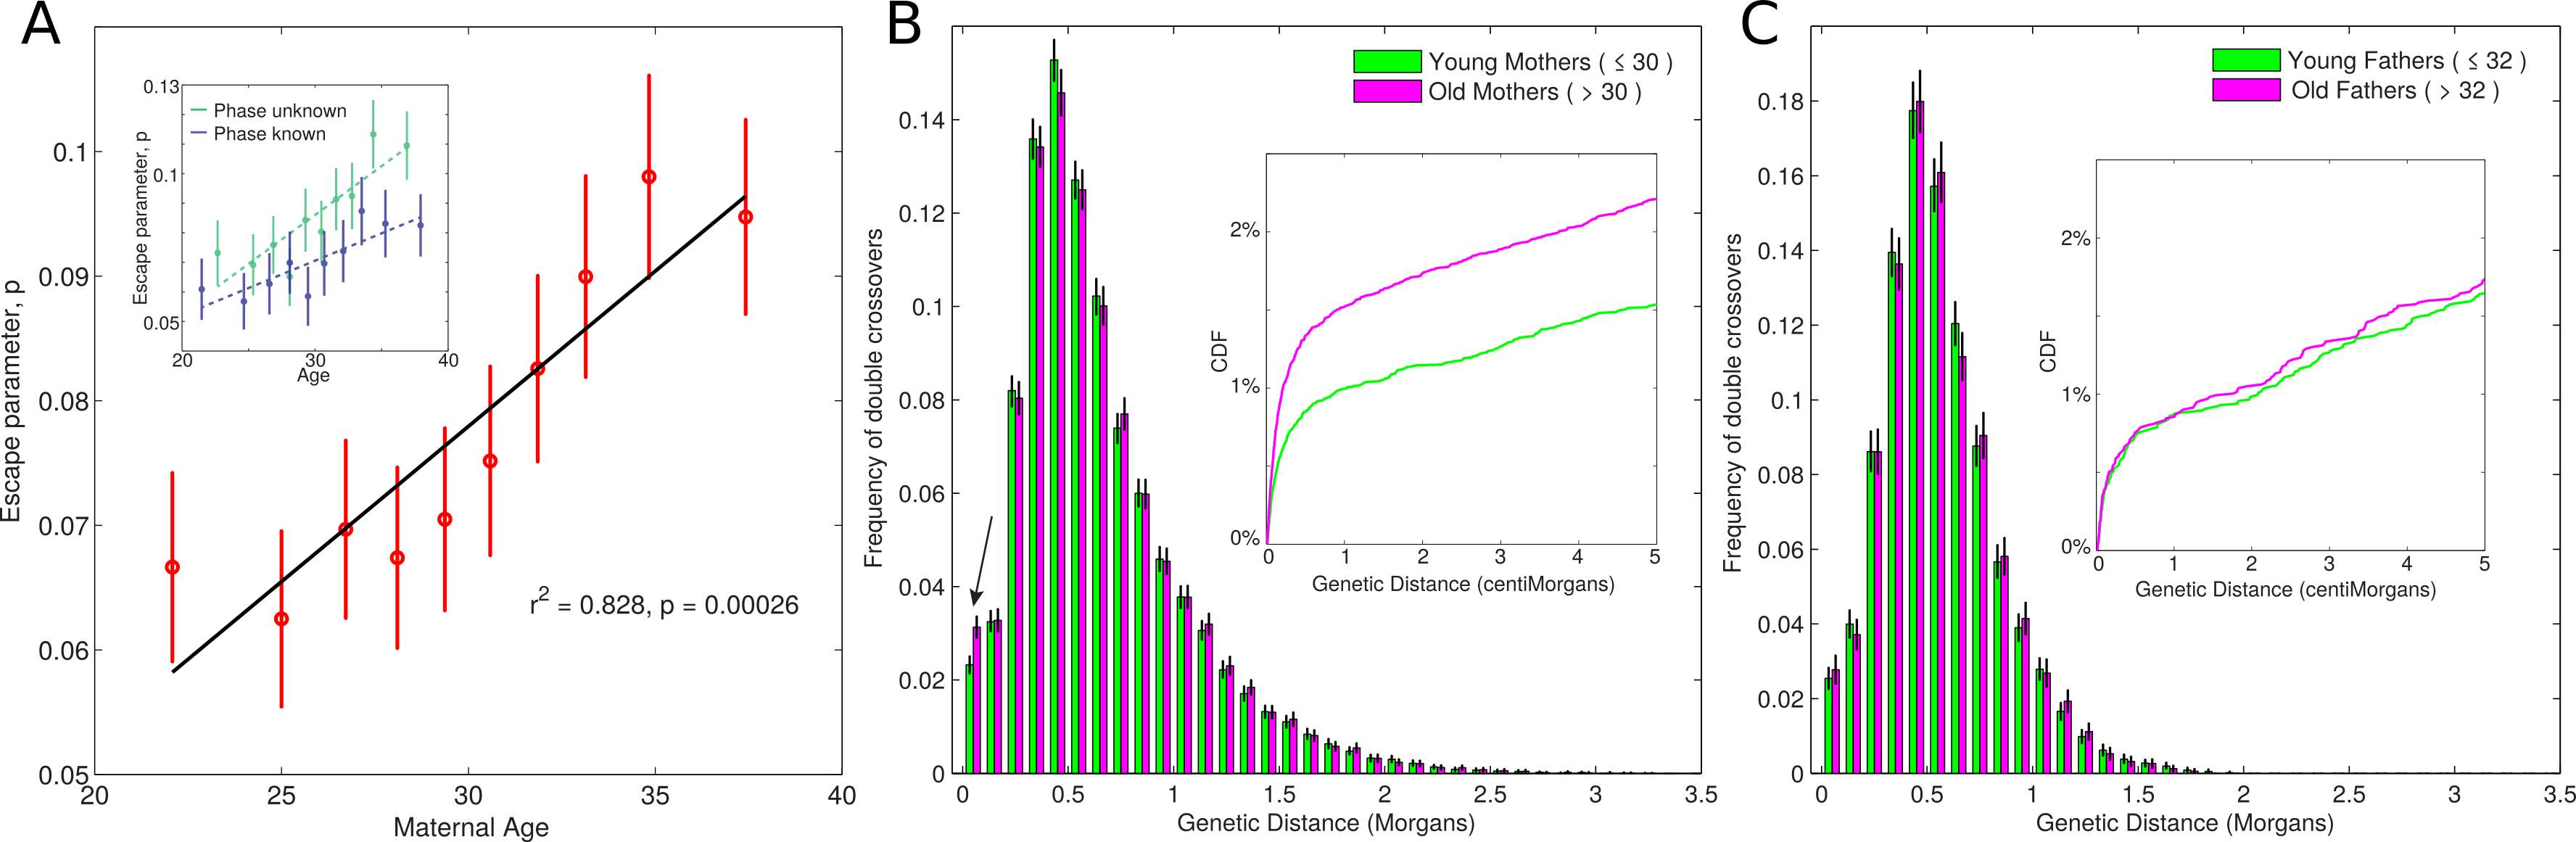
\includegraphics[width=\textwidth]{cointEscape/figs/Figure4.png}
    %\vspace{-20pt}
    \captionTitle{\textbf{Genetic map estimated from 23andMe data.}}{
        Genetic maps from the 23andMe data are shown in bold lines, whereas the genetic maps from deCODE are shown as thin lines.
        Separate maps are shown for females (red), males(blue), and sex-averaged (black).
        Also shown are regions highlighted in grey that represent gaps in the reference assembly. 
        For PAR1, we are showing data derived from Duffy\cite{Duffy2006} for comparison.
        As the deCODE maps cover a slightly smaller physical region than the 23andMe maps, the deCODE maps have been shifted slightly upwards to aid visual comparison.
        Specifically, the deCODE map has been aligned with the 23andMe map at the first physical position within the deCODE map.
        The locations of the alignments are indicated by small circles that can be most clearly seen on the smaller chromosomes.  
       \label{fig:cointFS4}}
\end{figure}

\begin{figure}[!h]
    %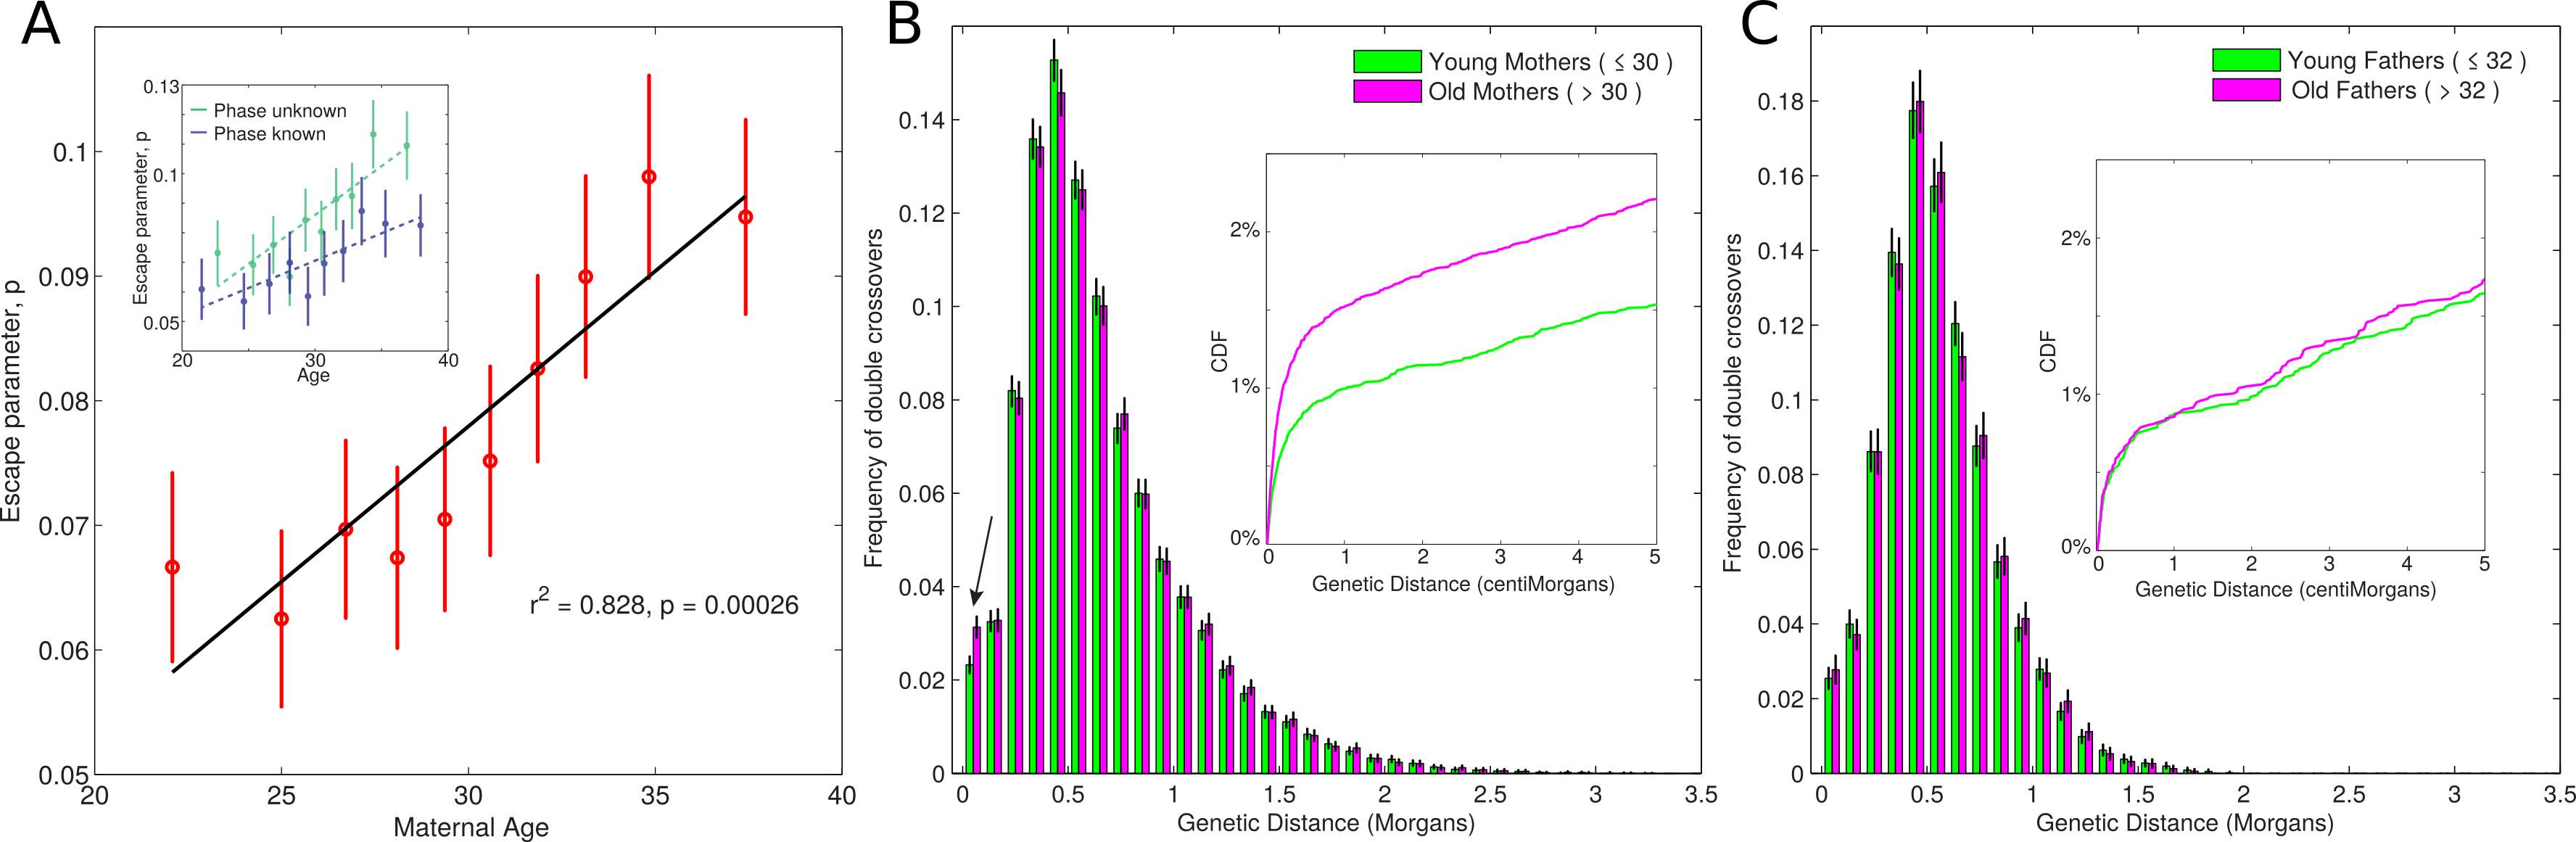
\includegraphics[width=\textwidth]{cointEscape/figs/Figure4.png}
    %\vspace{-20pt}
    \captionTitle{\textbf{The relationship between chromosome length and recombination.}}{ 
        The top row shows the correlation between physical length and map length for females (left), males (center), and sex averaged (right), with a linear fit included for the 23andMe map (red) and the deCODE map (blue).
        The bottom row shows the relationship between physical length and average recombination rate with a quadratic fit. 
        Note that chromosome X has been included in the female plots, but was excluded from the regressions.  
       \label{fig:cointFS5}}
\end{figure}

\begin{figure}[!h]
    %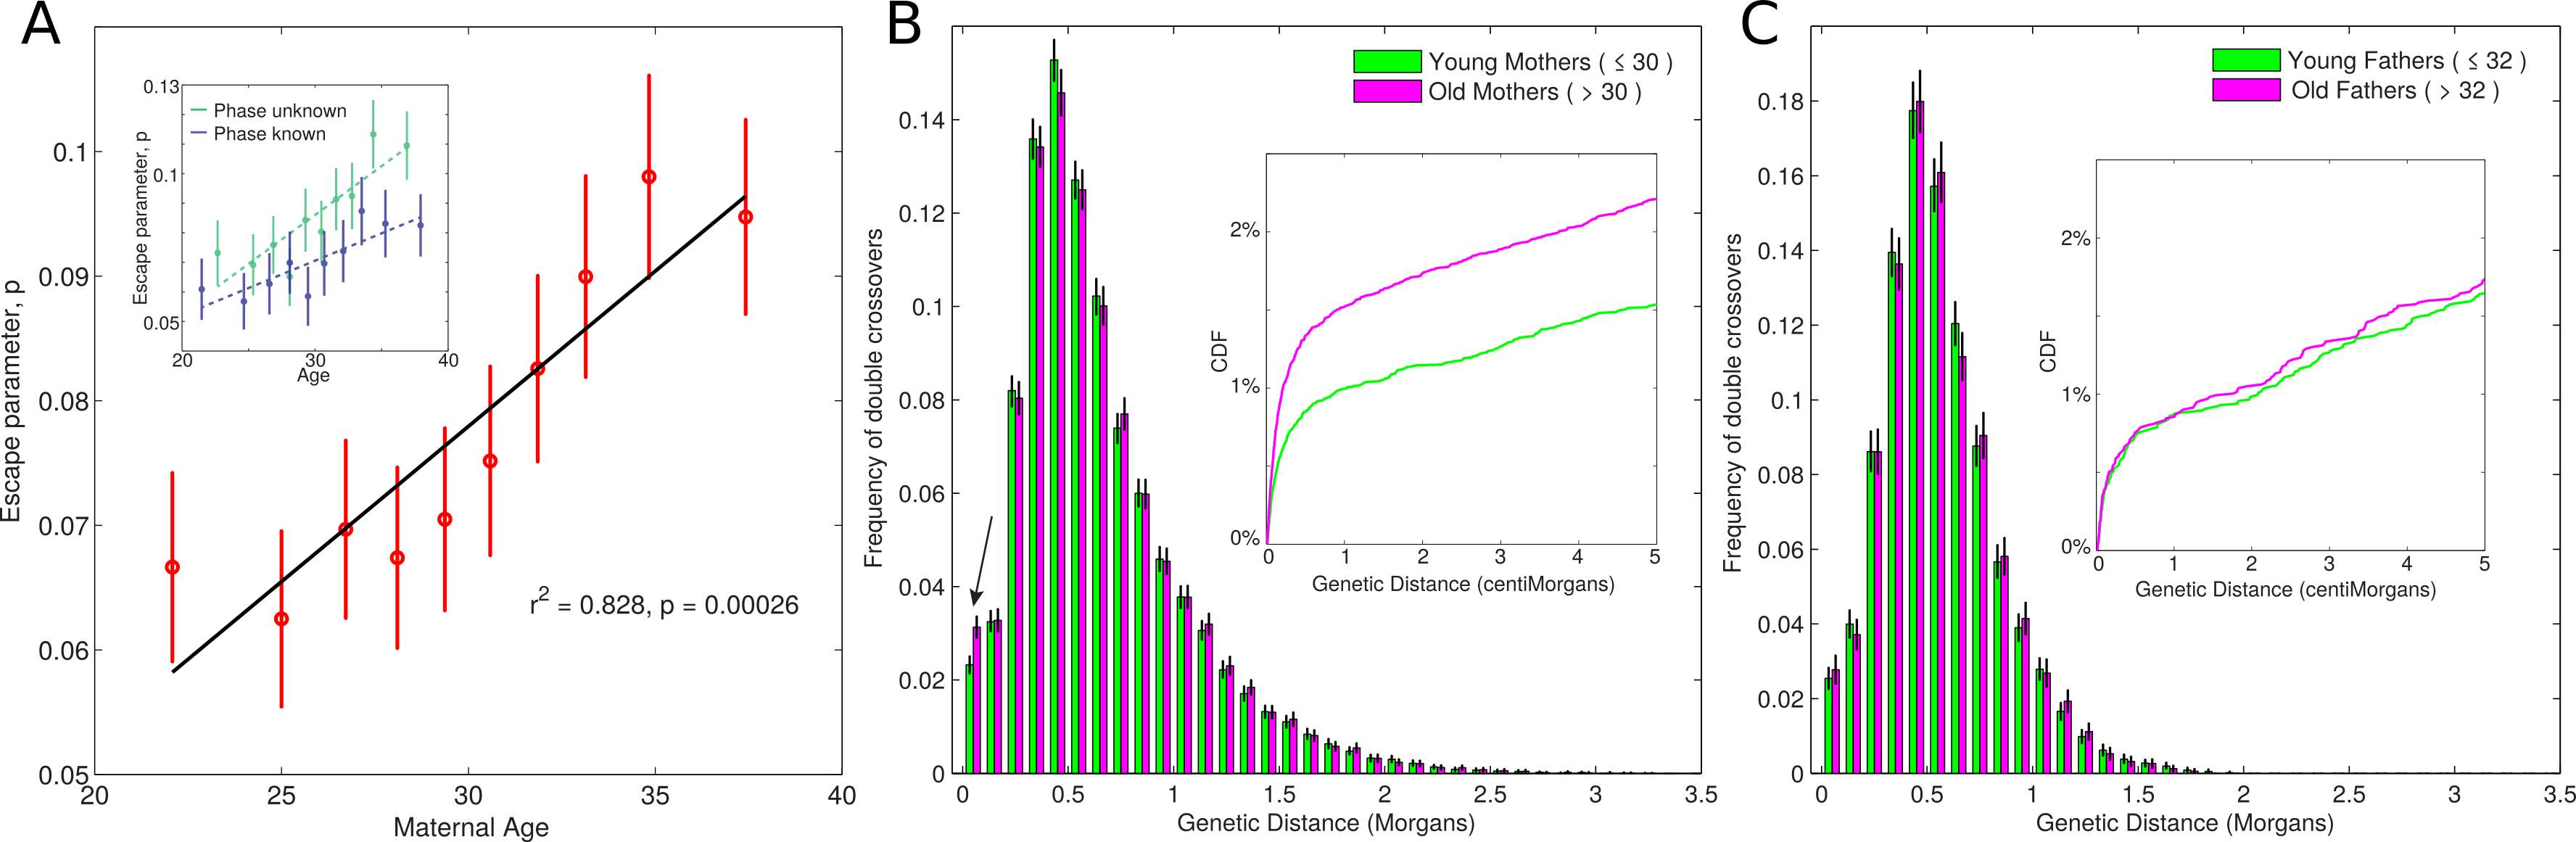
\includegraphics[width=\textwidth]{cointEscape/figs/Figure4.png}
    %\vspace{-20pt}
    \captionTitle{\textbf{Number of autosome recombination events verses parental age}}{
        for females (left) and males (right). 
        A linear least-squares fit is indicated by a black line.
        The least-squares fit equation given in the legend together with a p-value for the non-constant term.   
       \label{fig:cointFS6}}
\end{figure}

\begin{figure}[!h]
    %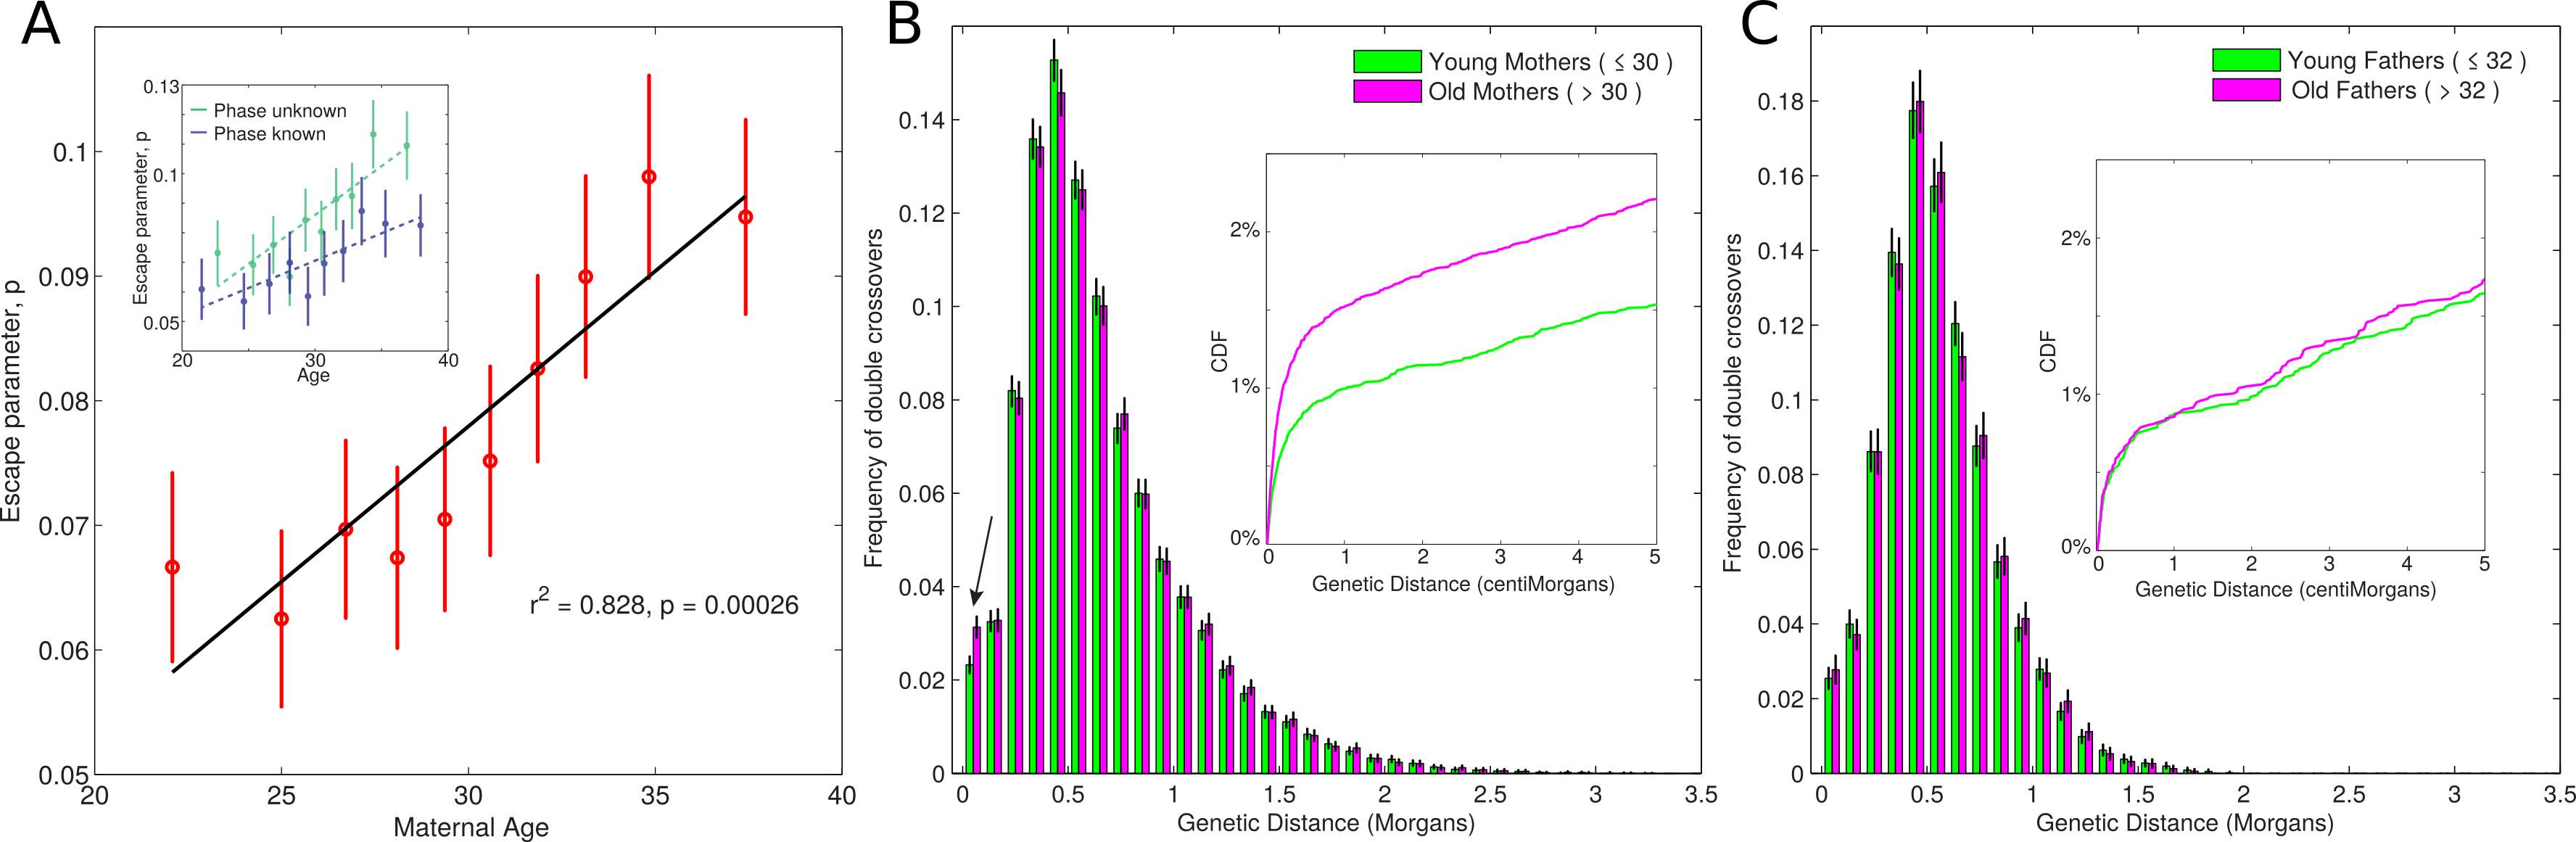
\includegraphics[width=\textwidth]{cointEscape/figs/Figure4.png}
    %\vspace{-20pt}
    \caption[\textbf{Hotspot usage between sexes.}]{
        A) Hotspot usage estimated in females (left) and males(right). 
        The MLE estimate for each individual is indicated by a circle, with a 95\% confidence interval indicated by the shaded area.
        The median MLE estimate for each sex is indicated by a vertical black line.
        B) Hotspot usage by parental age for females(left) and males (right).
        For each plot a logistic regression is also shown, with the p-value for the non-constant term given in the title.  
       \label{fig:cointFS7}}
\end{figure}

\begin{figure}[!h]
    %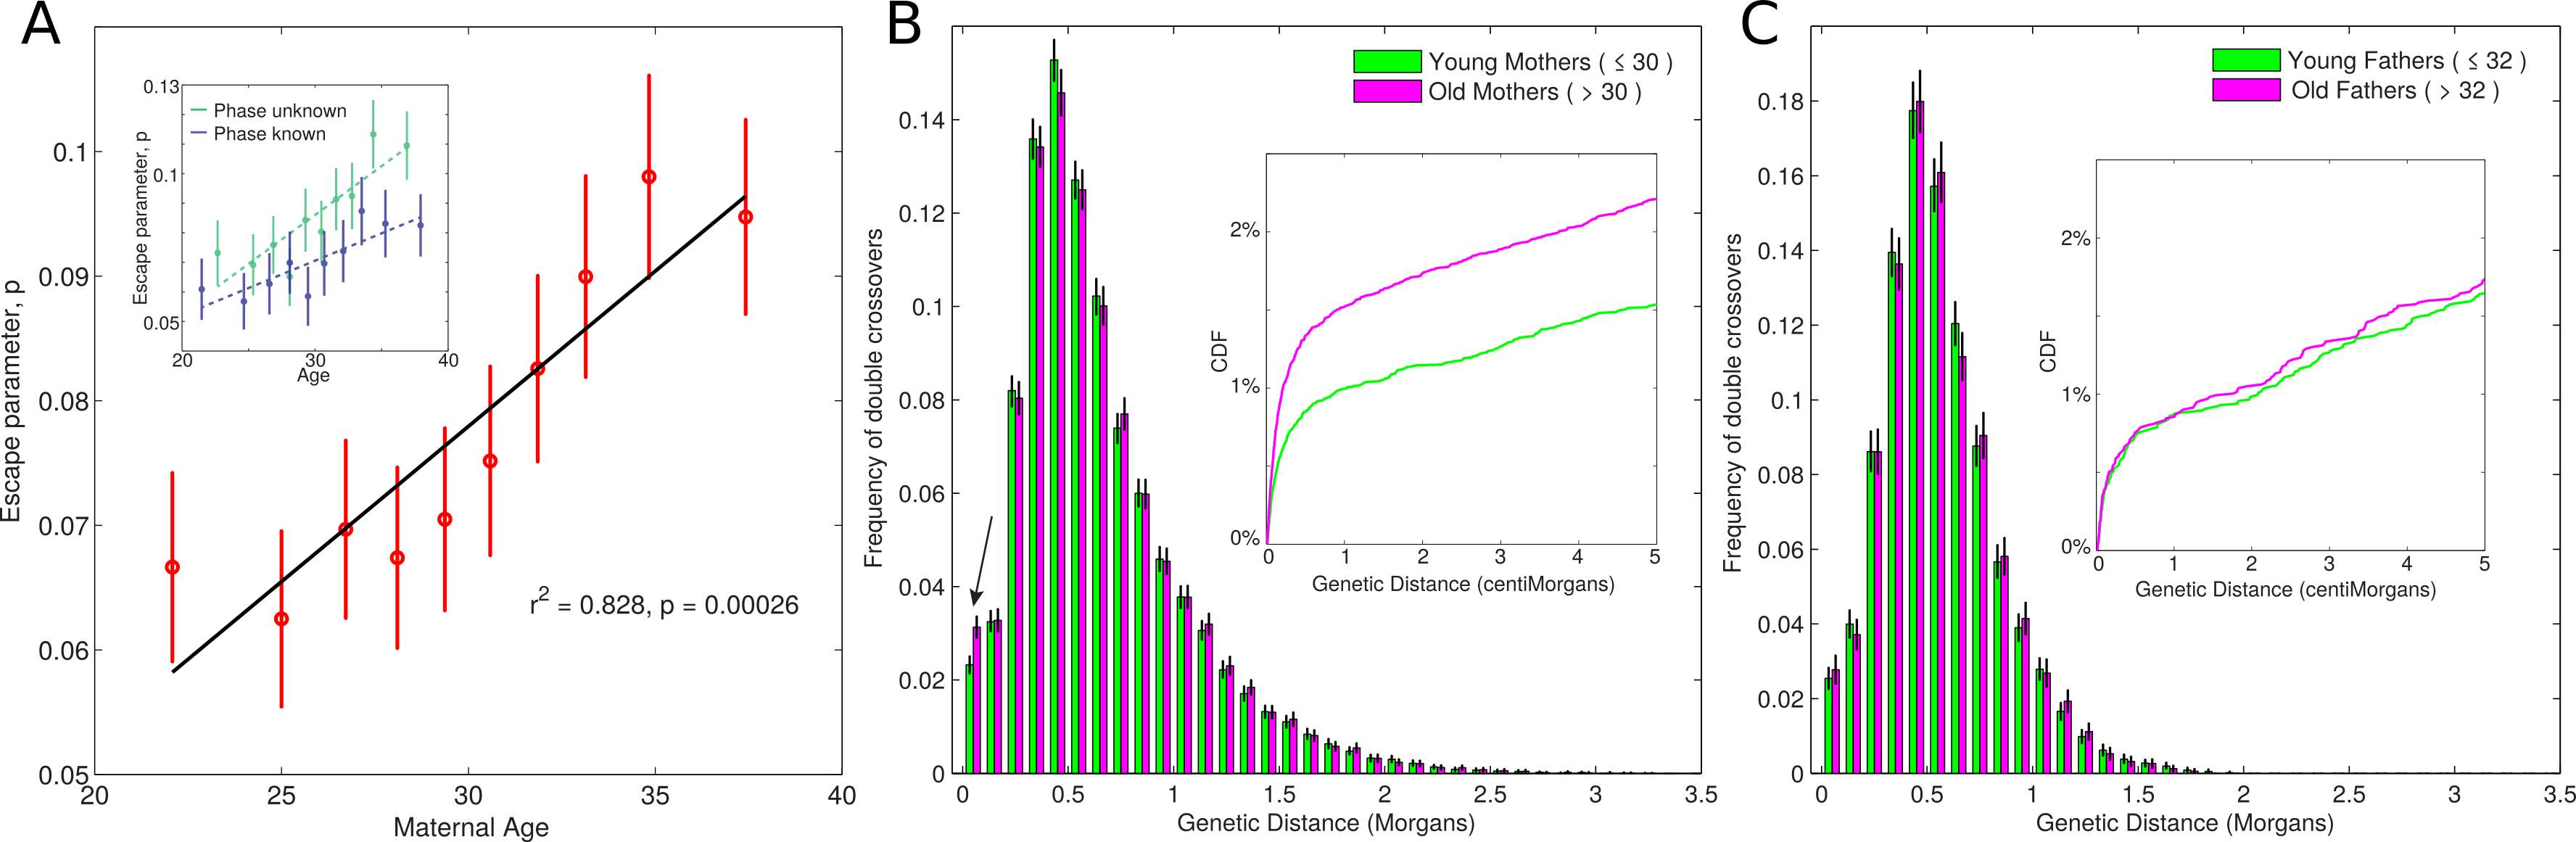
\includegraphics[width=\textwidth]{cointEscape/figs/Figure4.png}
    %\vspace{-20pt}
    \caption[\textbf{The relationship between map length and interference parameters.}]{ 
        A) The relationship between chromosome map length and the interference parameter, $\nu$.
        B) The relationship between chromosome map length and the escape parameter, $p$.
        Linear fits are shown for females (red), males (blue), and the data combined across sexes (black).
        In both plots, the chr21 estimate in males has been excluded.  
       \label{fig:cointFS8}}
\end{figure}

\begin{figure}[!h]
    %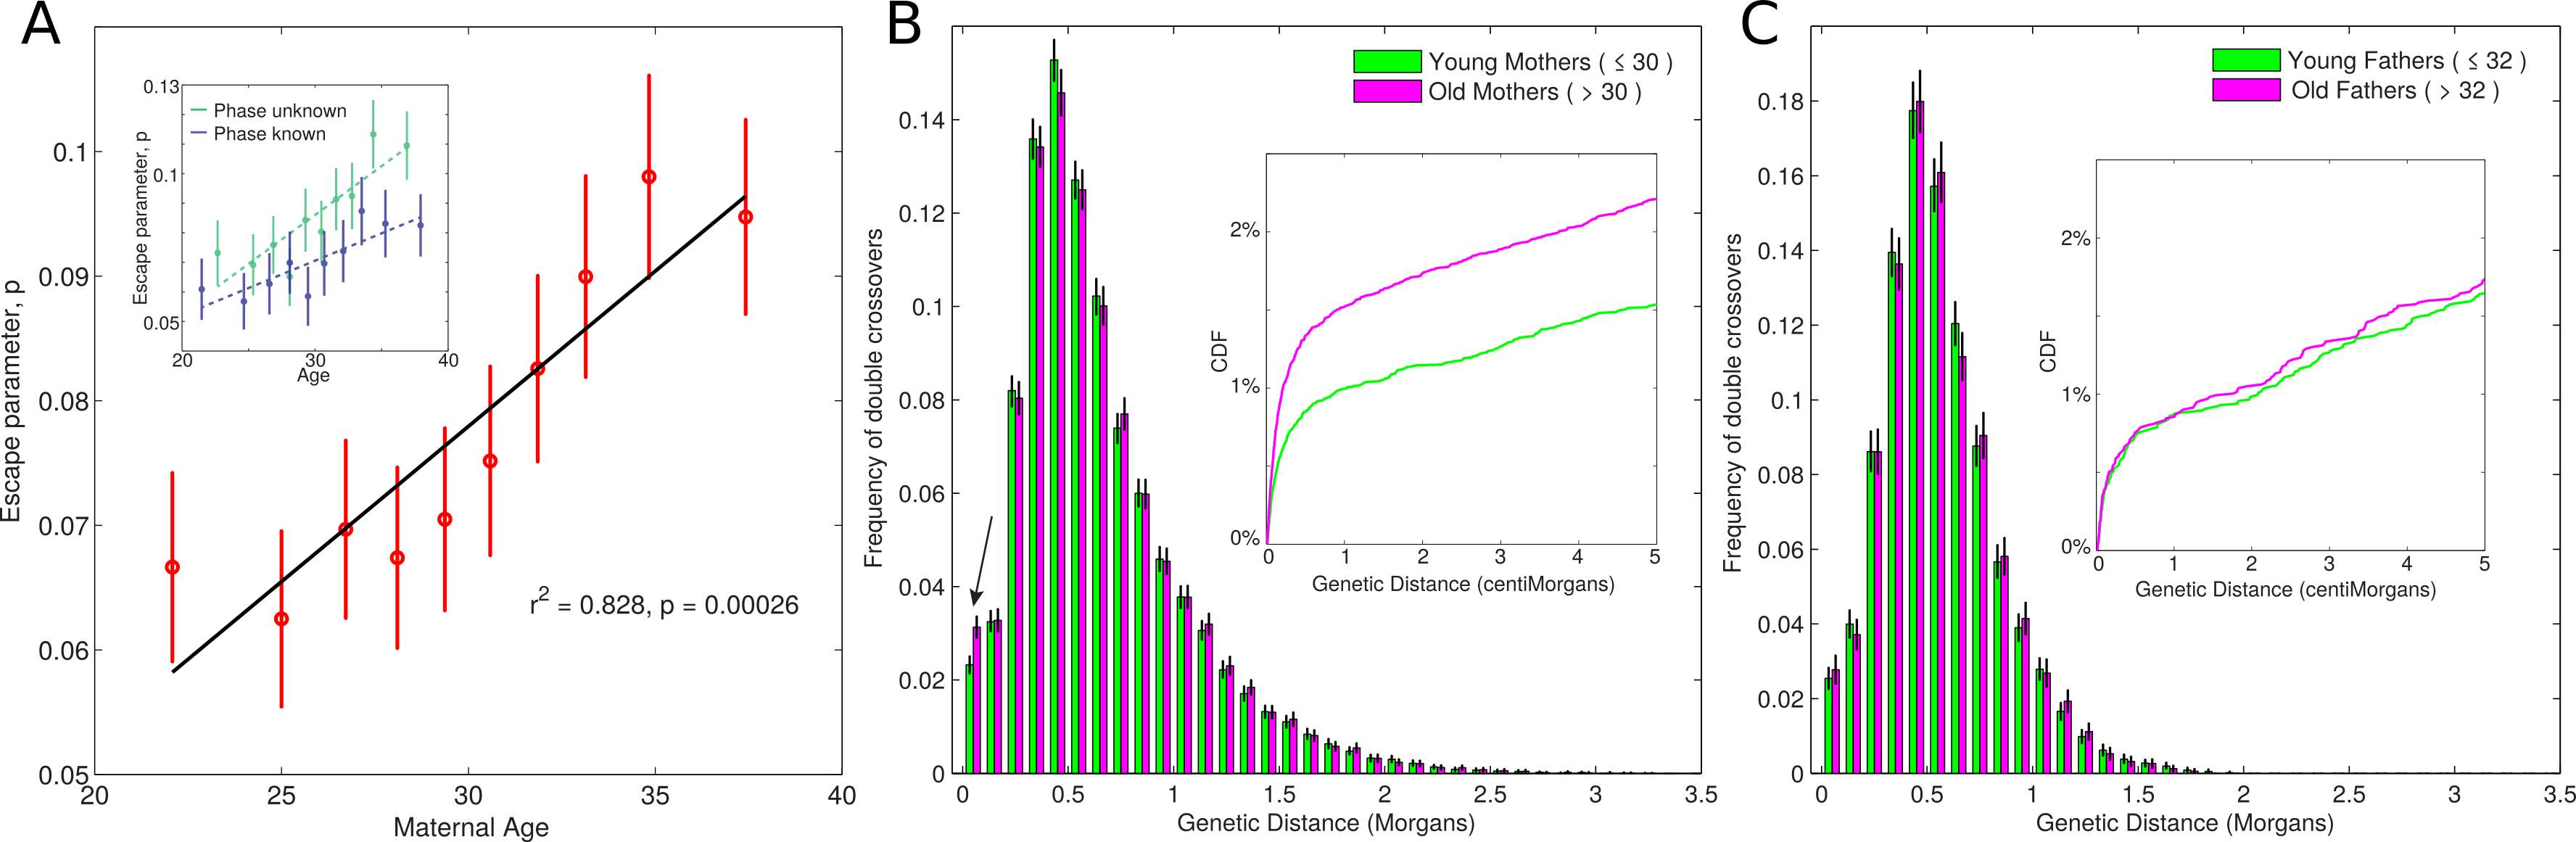
\includegraphics[width=\textwidth]{cointEscape/figs/Figure4.png}
    %\vspace{-20pt}
    \captionTitle{\textbf{Interference parameters as a function of age.}}{
        Females and males are shown on the top and bottom rows respectively. 
        Estimates of the interference parameter, $\nu$, are shown on the left, whereas estimates of the escape parameter, $p$, are shown on the right.
        Error bars show 95\% confidence intervals.  
       \label{fig:cointFS9}}
\end{figure}

\begin{figure}[!h]
    %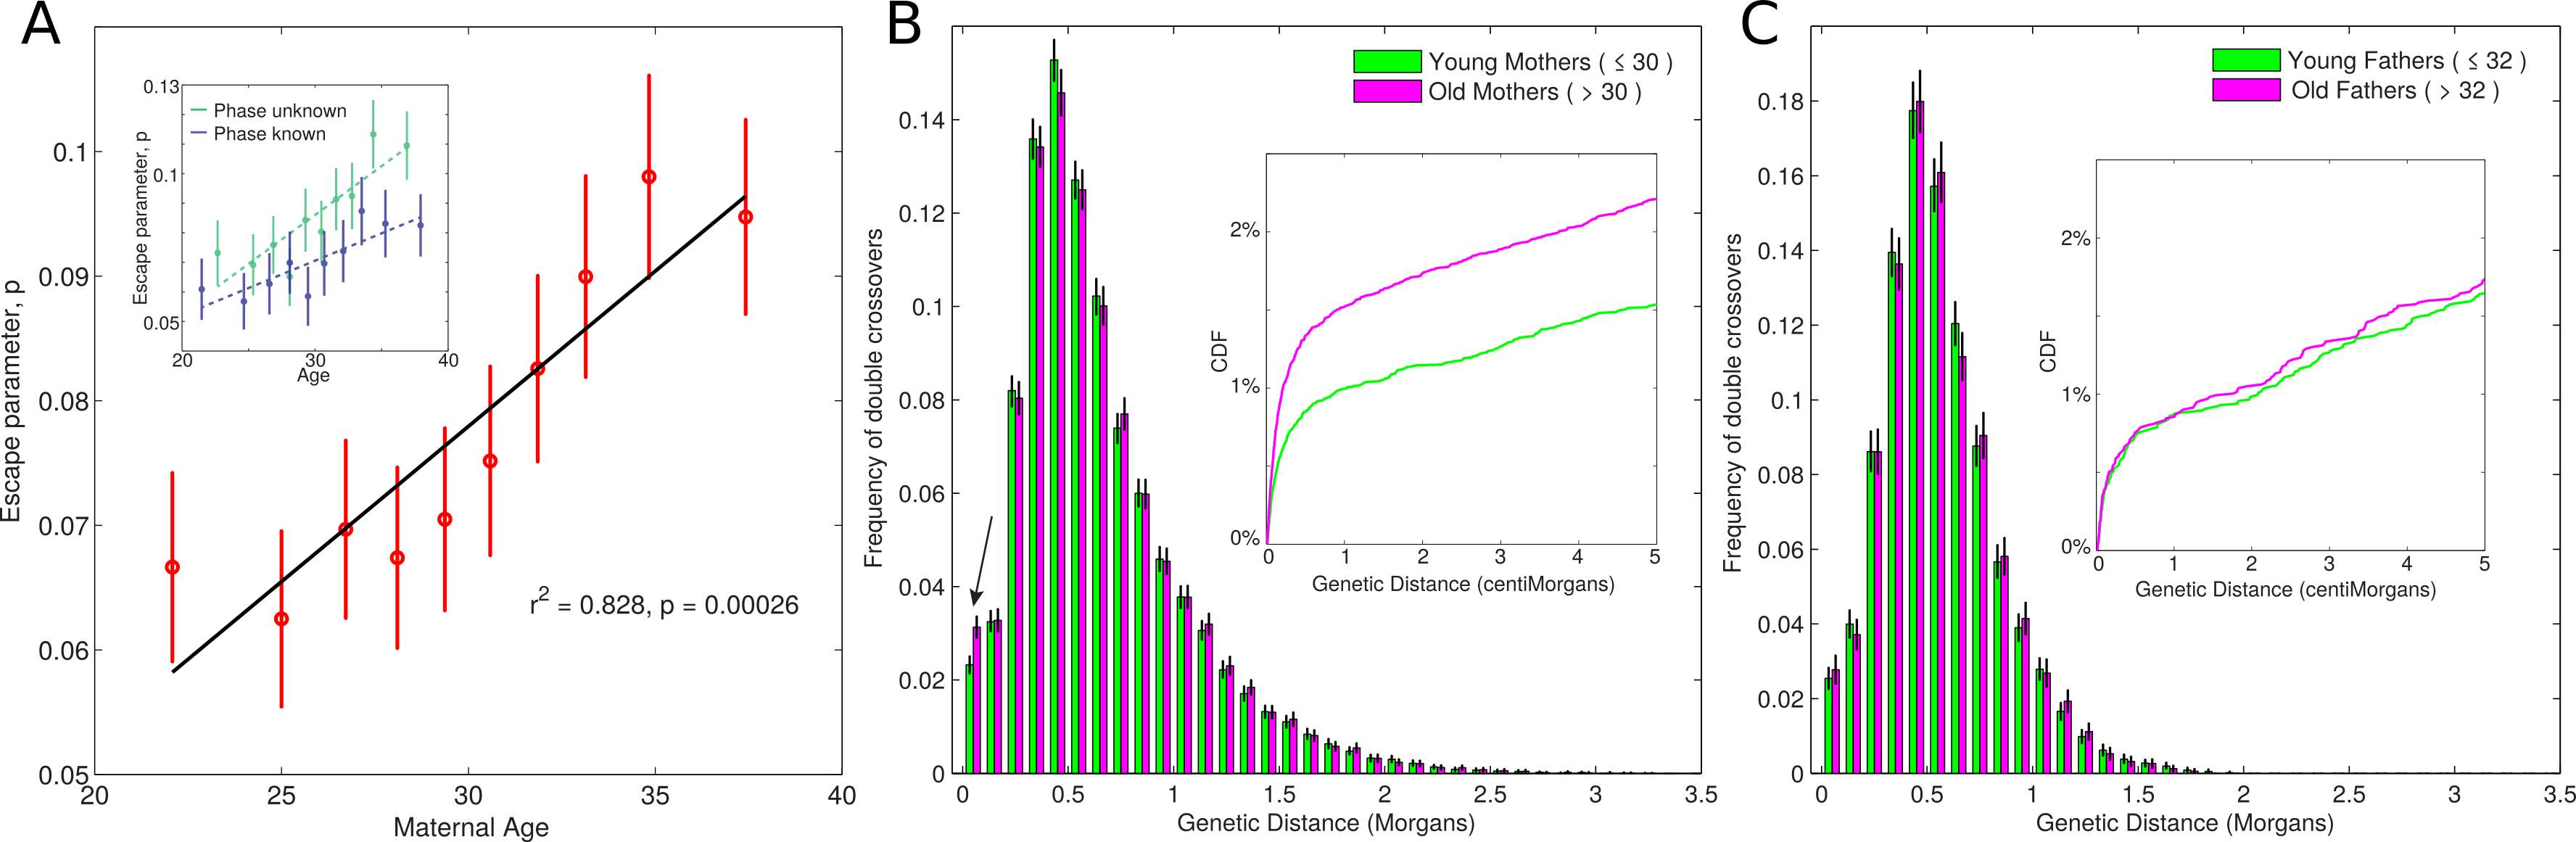
\includegraphics[width=\textwidth]{cointEscape/figs/Figure4.png}
    %\vspace{-20pt}
    \captionTitle{\textbf{Interference parameters by age}}{,
        having divided the data in 5 or 20 age quantiles.
        Error bars show 95\% confidence intervals.  
       \label{fig:cointFS10}}
\end{figure}

\begin{figure}[!h]
    %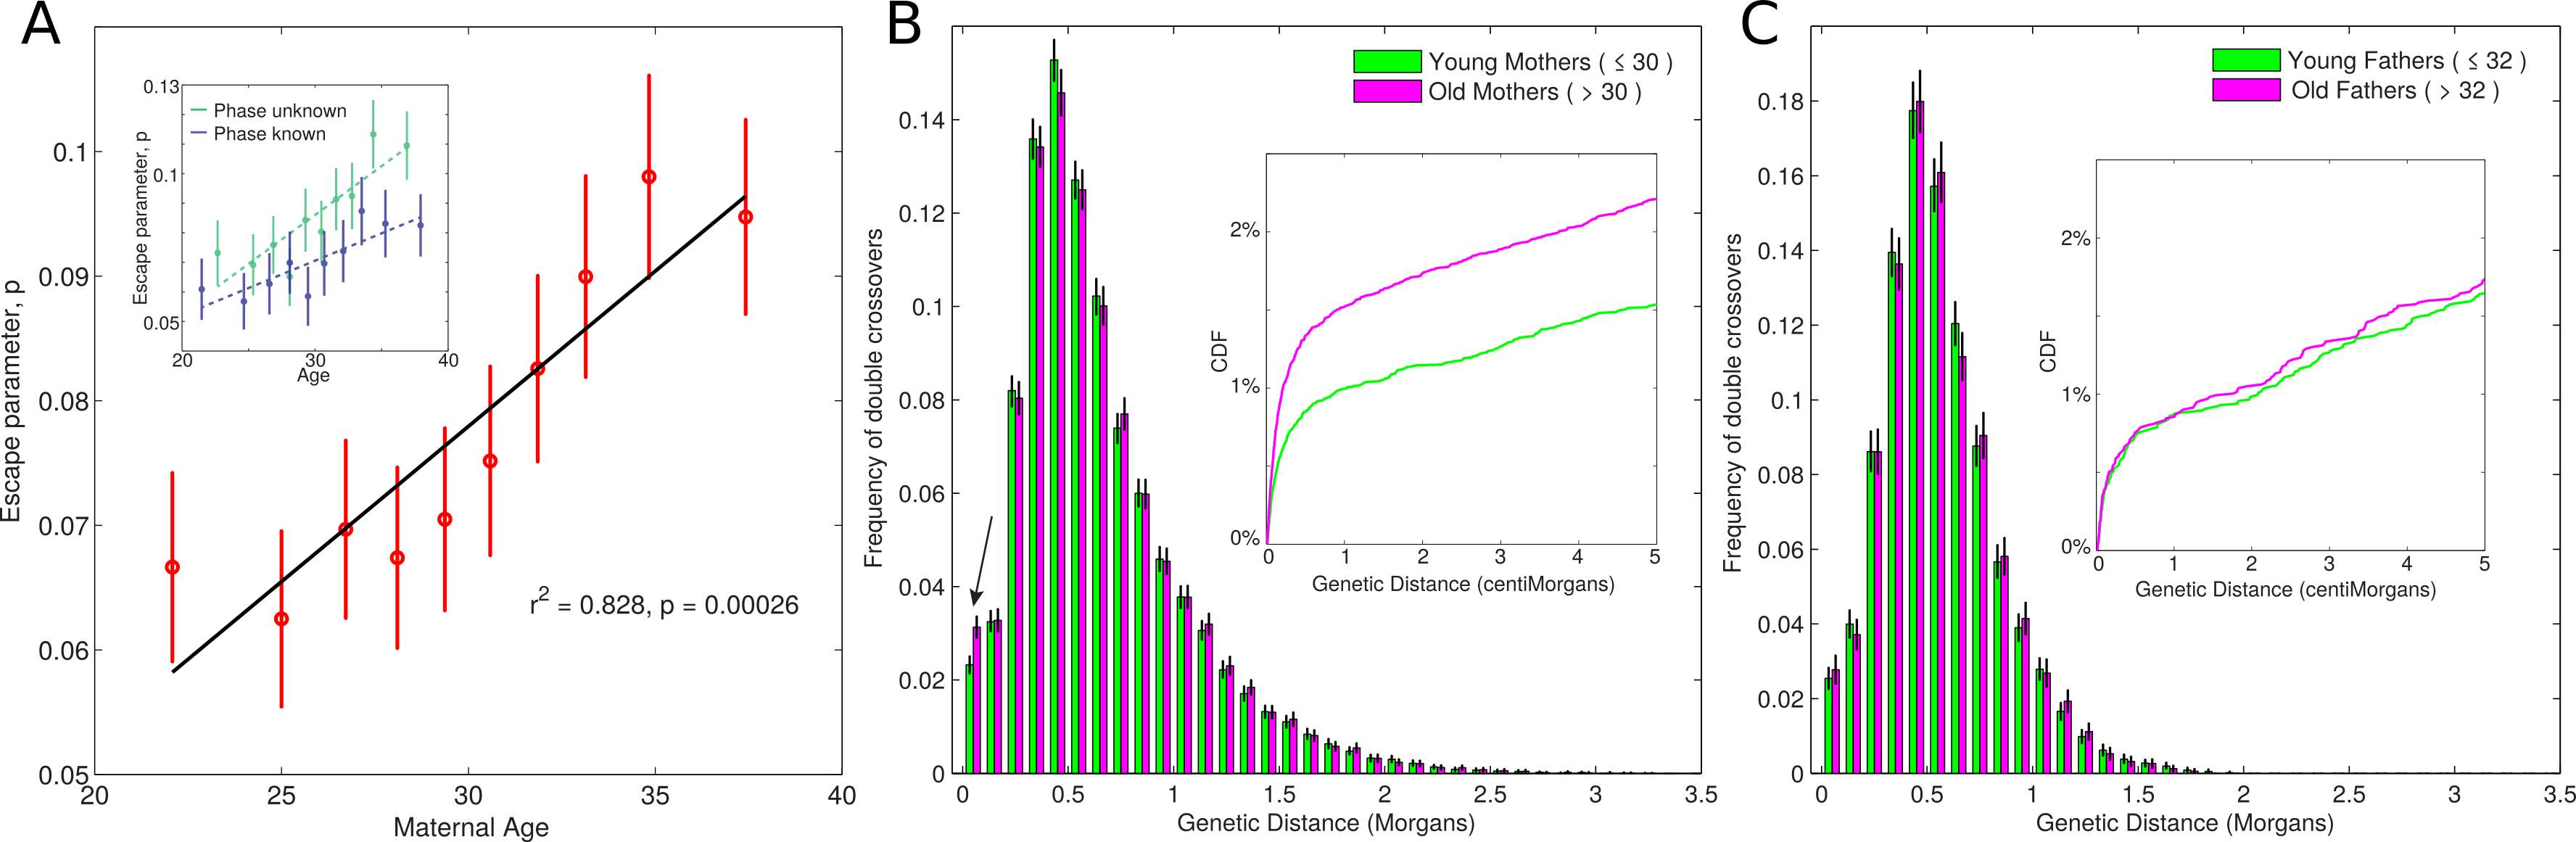
\includegraphics[width=\textwidth]{cointEscape/figs/Figure4.png}
    %\vspace{-20pt}
    \caption{\textbf{Interference parameters by age and phase.}}{ 
        Interference parameters by age, having estimated the interference parameters for phase-known and phase-unknown groups separately.  
       \label{fig:cointFS11}}
\end{figure}

\begin{figure}[!h]
    %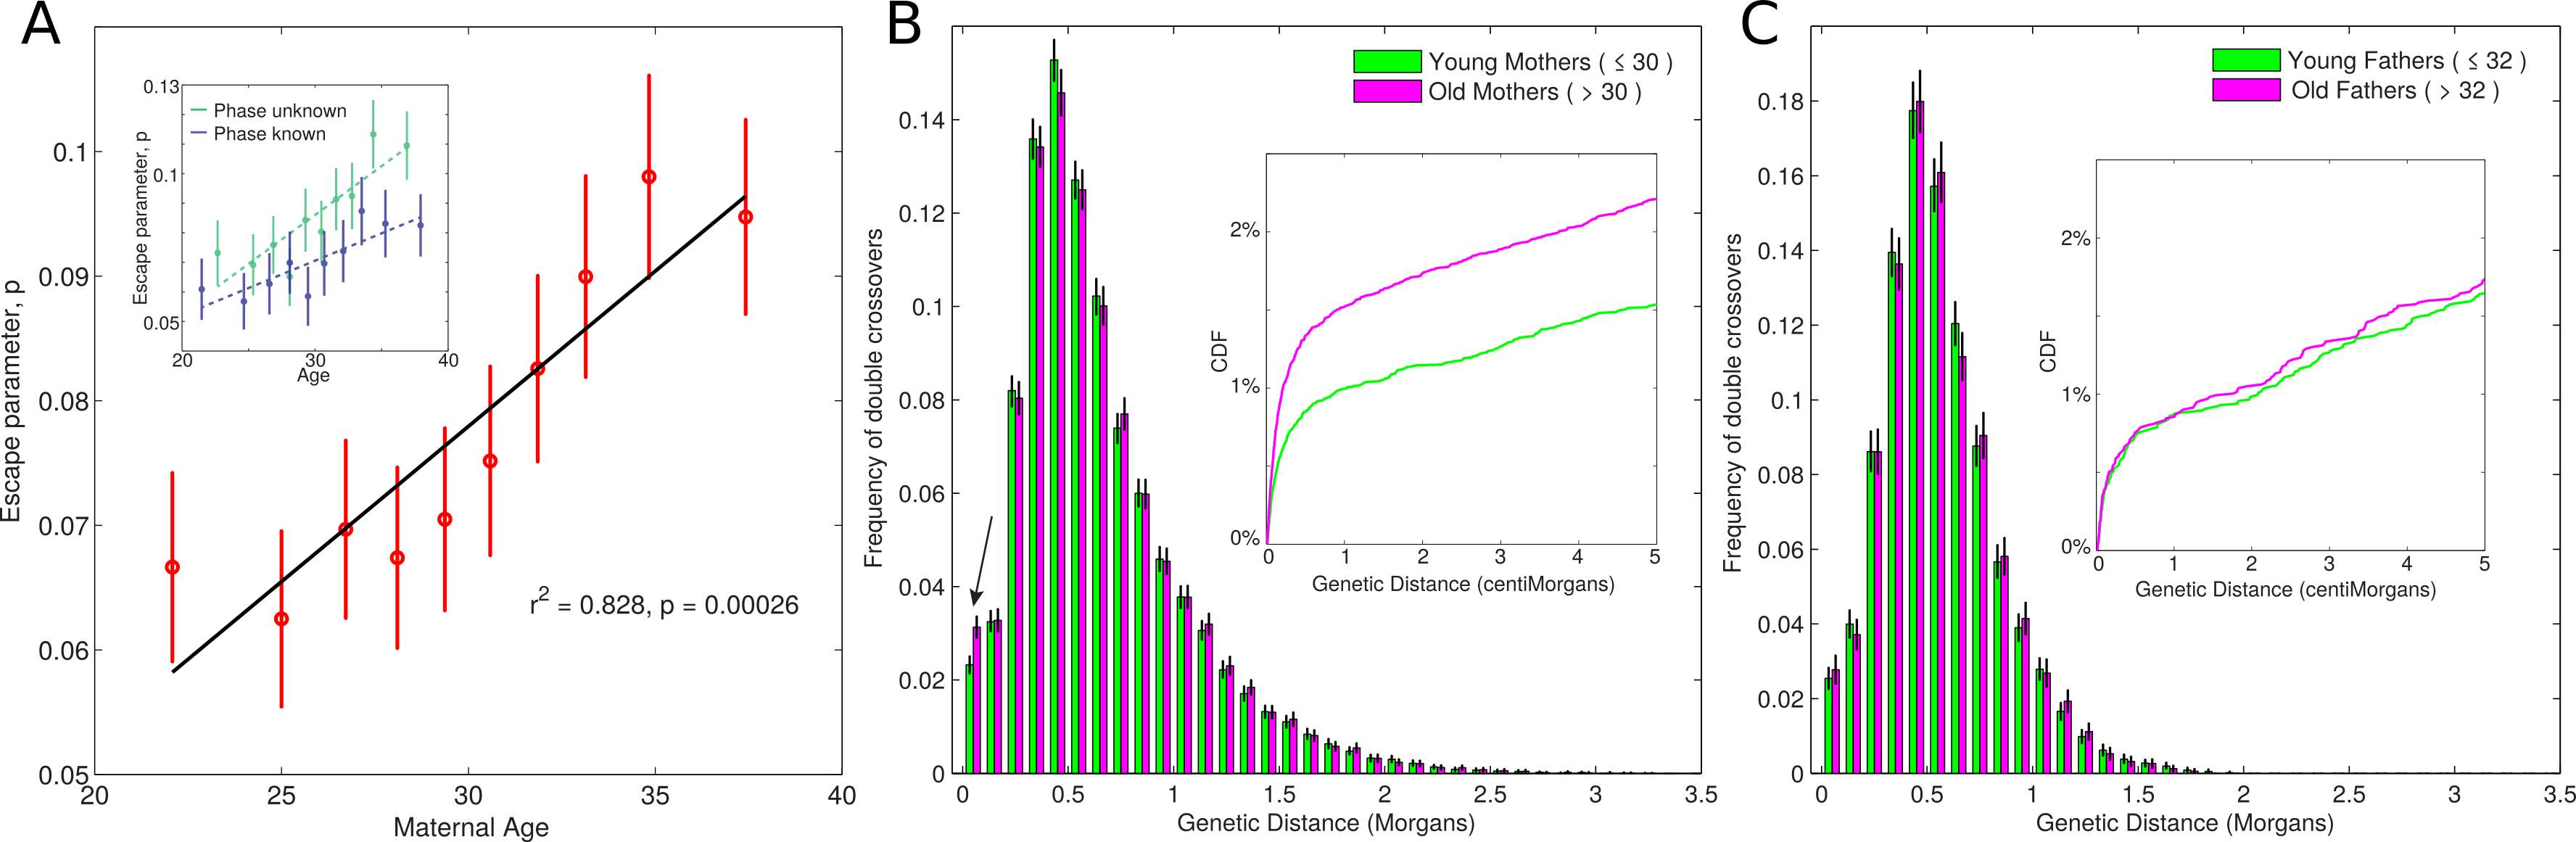
\includegraphics[width=\textwidth]{cointEscape/figs/Figure4.png}
    %\vspace{-20pt}
    \captionTitle{\textbf{Interference parameters as a function of age, following stratified sampling.}}{
        Females and males are shown on the top and bottom rows respectively.
        Estimates of the interference parameter, $\nu$, are shown on the left, whereas estimates of the escape parameter, $p$, are shown on the right.
        Error bars show 95\% confidence intervals.  
       \label{fig:cointFS12}}
\end{figure}

\begin{figure}[!h]
    %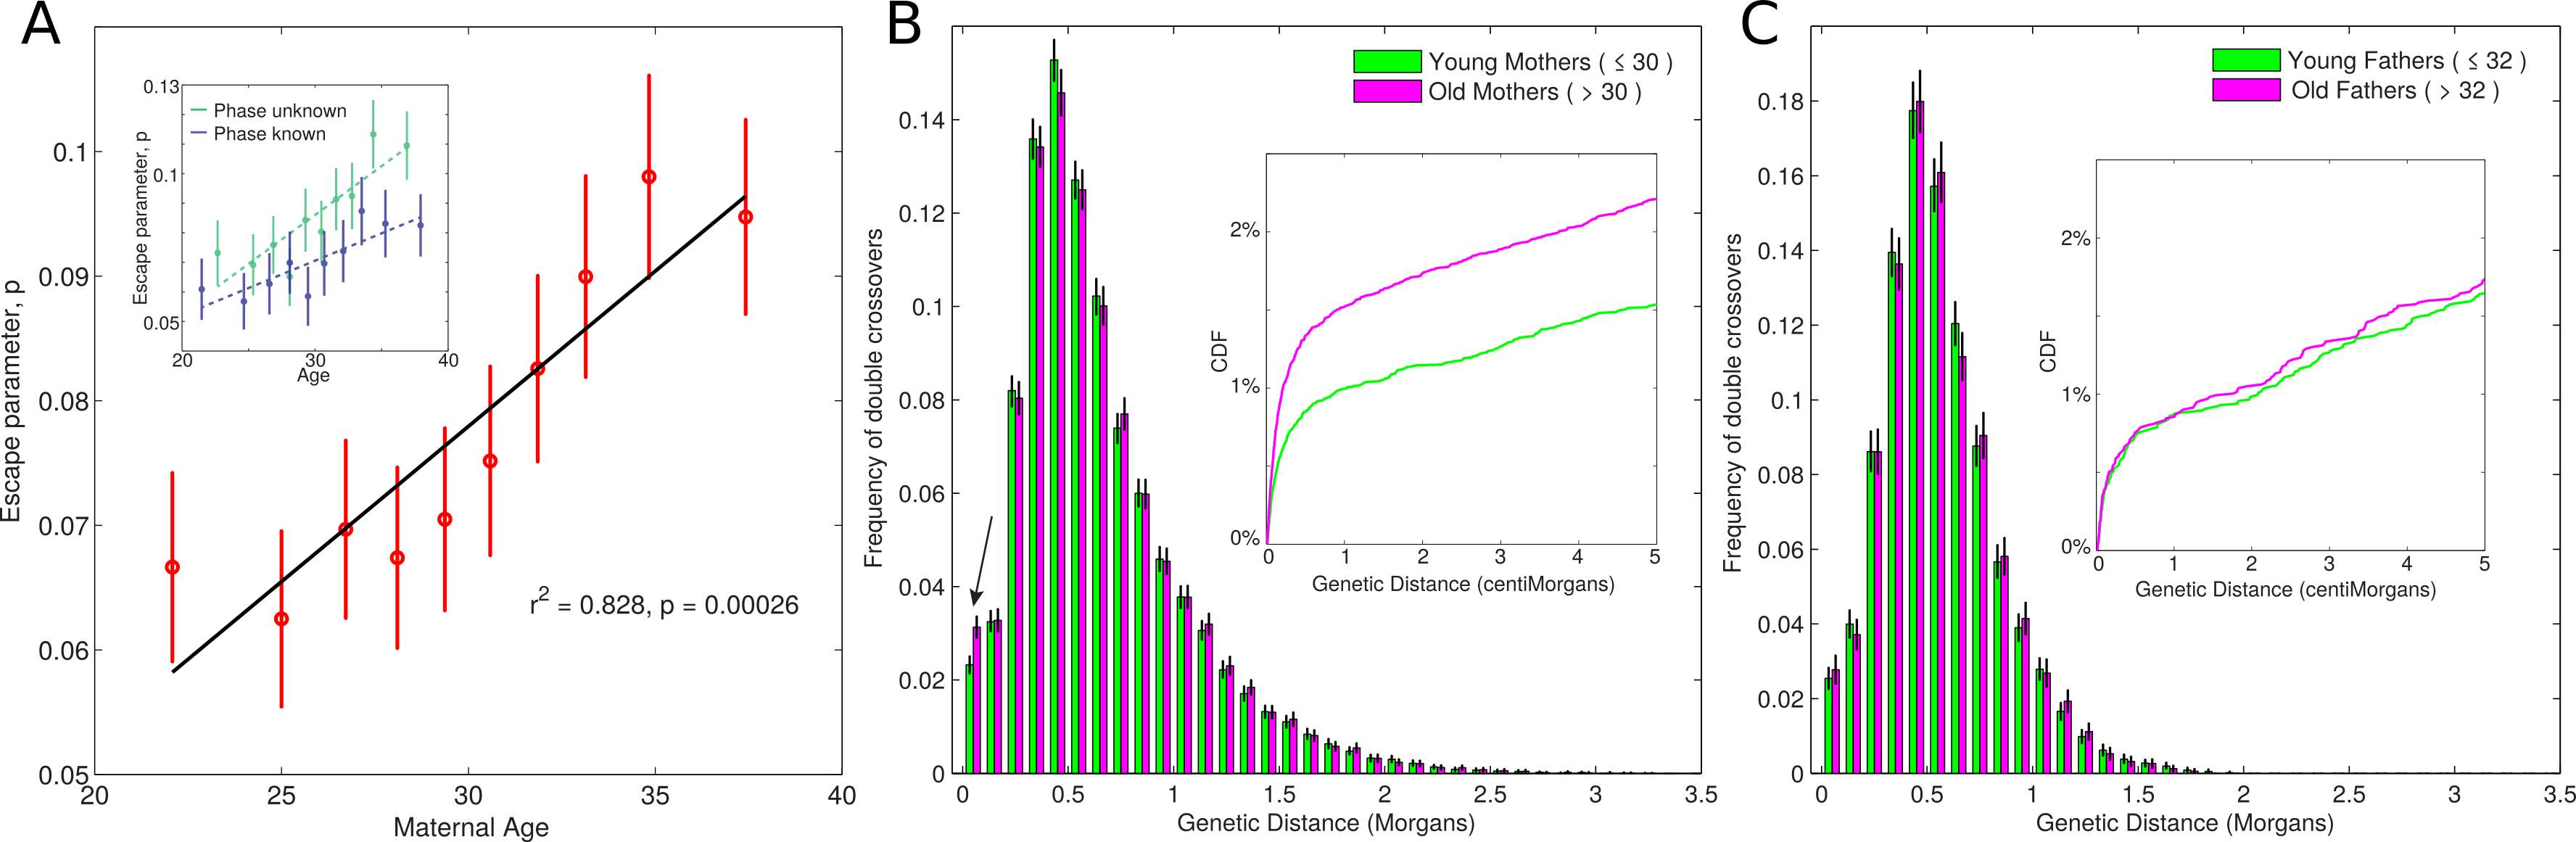
\includegraphics[width=\textwidth]{cointEscape/figs/Figure4.png}
    \vspace{-20pt}
    \captionTitle{\textbf{Model fit for tightly clustered events}}{
        in females (A) and males (B).
        The figure shows the empirical cumulative distribution function for young (green line) and old (magenta line) mothers/fathers, and compares to that obtained via simulation under the interference free model (black dotted line), the Gamma simple interference model (black dashed line), and the Housworth-Stahl interference escape model (solid black line), with parameters were taken from Supplementary Table 7.
        The figure is shown on a log-log scale to emphasize the short inter-crossover distances.  
       \label{fig:cointFS13}}
\end{figure}

\begin{figure}[!h]
    %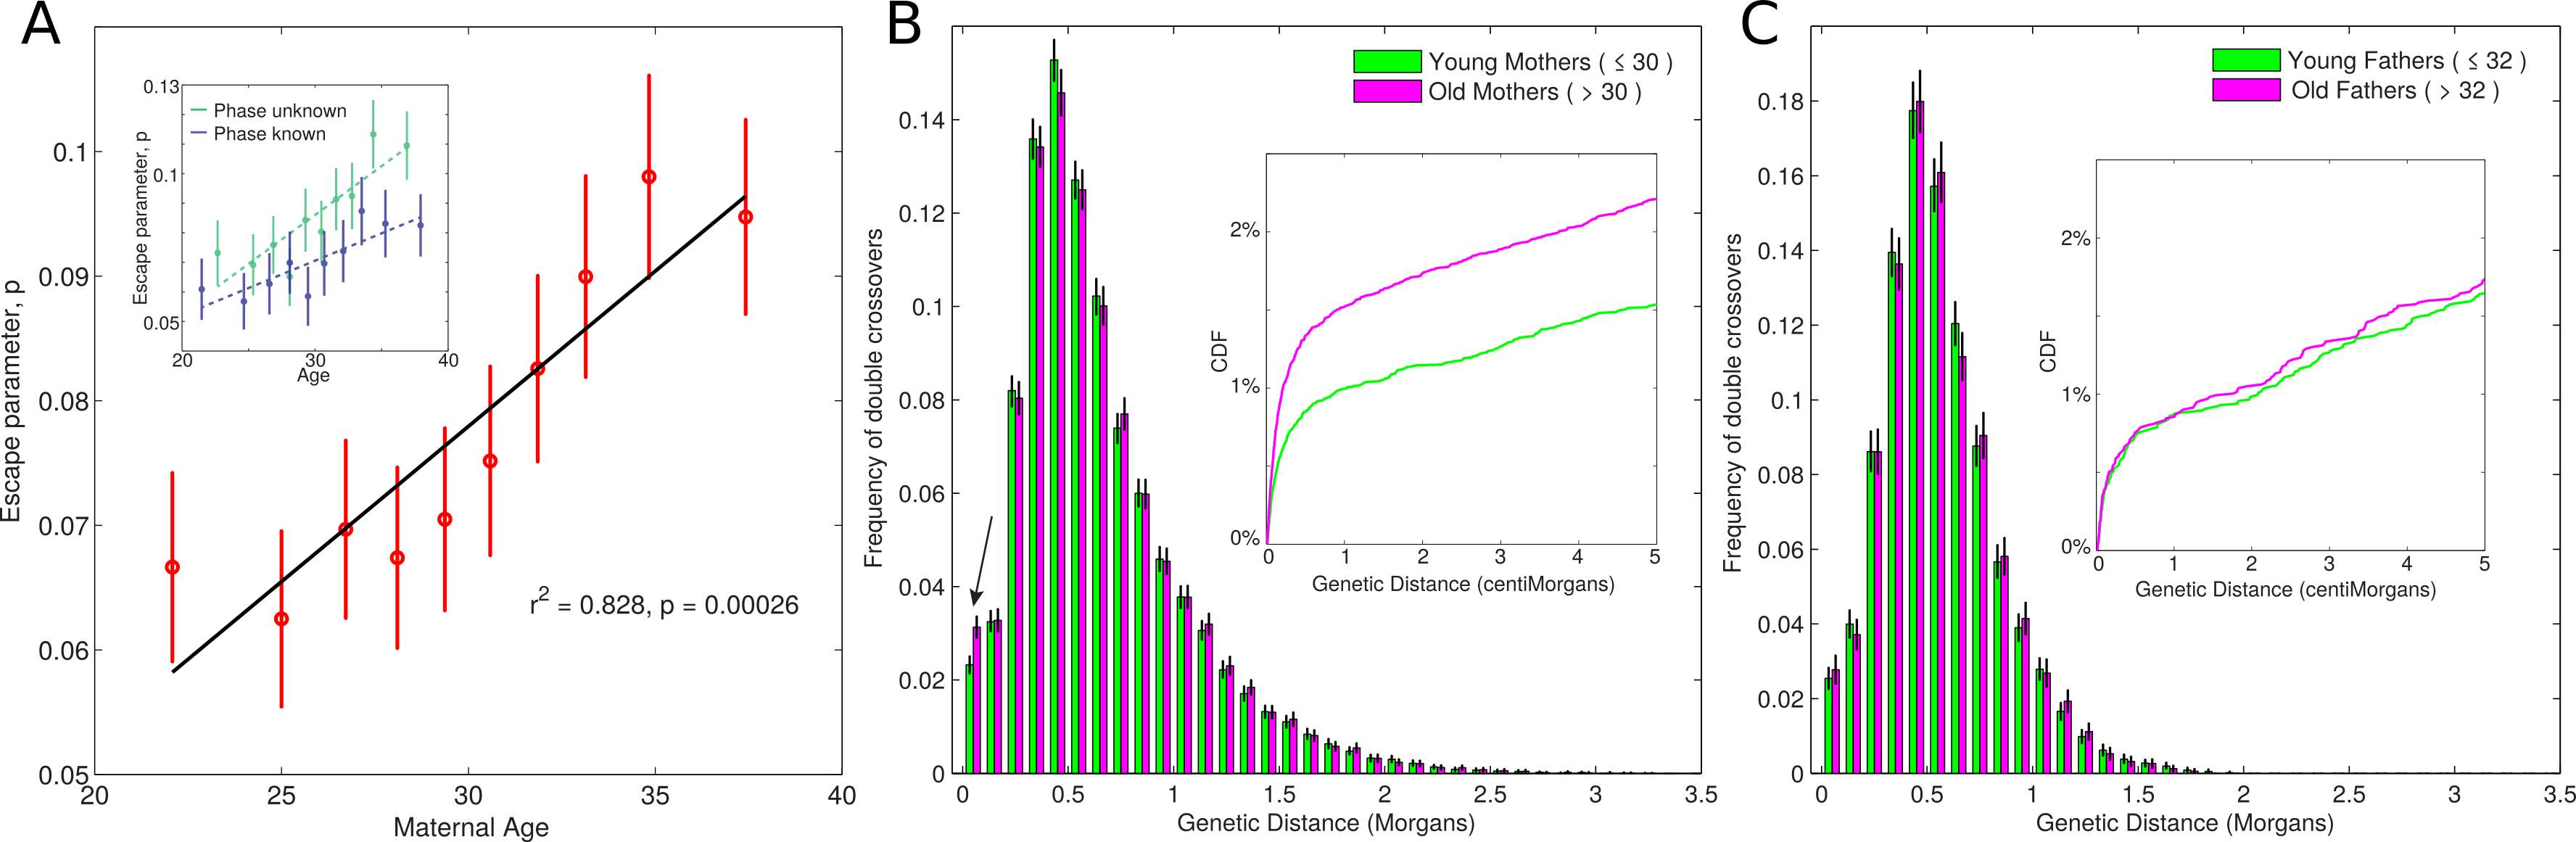
\includegraphics[width=\textwidth]{cointEscape/figs/Figure4.png}
    \vspace{-20pt}
    \captionTitle{\textbf{Interference parameters estimated for a strictly filtered dataset.}}{
        In this case, all crossover events were required at least 10 supporting informative sites (compared to 3 in the main dataset), no two events within a single family were allowed to be within 5 SNPs of each other (compared to 1 in the main dataset), and no more than 4 events within 1 Mb of each other were allowed across the whole dataset (and compared to 14 in the main dataset, which corresponds to the 99.9\textsuperscript{th} percentile).
        After this very strict filtering, the deviation from the Housworth-Stahl interference escape model is much less pronounced at short scales (right hand panels), but the association between interference escape and maternal  
        age remains strong (2\textsuperscript{nd} panel from top left).   
       \label{fig:cointFS14}}
\end{figure}

\clearpage
\section{Supplementary Tables}


\begin{table}[!h] \centering
    \begin{tabular}{|c|c|c|c|} 
        \hline Pedigree Type & Description & Before Filtering & After Filtering \\ \hline
        1 & 2 parents, 2 children & 3319 & 3307 \\
        2 & 2 parents, 3 children & 560 & 523 \\
        3 & 2 parents, 4 children & 89 & 80 \\
        4 & Quartet, with 2nd generation trio & 101 & 100 \\
        5 & Trio, with 2nd generation quartet & 201 & 199 \\
        \hline & \textbf{Total} & \textbf{4270} & \textbf{4209} \\
    \hline \end{tabular}
    \captionTitle{\textbf{Summary of dataset, before and after filtering.}}{
    \label{tab:cointTS1}}
\end{table}

\begin{table}[!h] \centering
    \begin{tabular}{|p{3cm}p{1.5cm}p{1.5cm}p{1.5cm}p{1.5cm}p{1.5cm}p{2cm}|}
        \hline 
    Population & Female \mbox{unphased} & Male \mbox{unphased} & Female phased & Male phased & Total Meioses & Percentage \\ \hline
    Europe & 5382 & 5508 & 1789 & 1641 & 14320 & 78.24\% \\
    Latino & 602 & 546 & 171 & 190 & 1509 & 8.25\% \\
    East Asia & 380 & 308 & 88 & 74 & 850 & 4.64\% \\
    None/Other & 198 & 268 & 68 & 109 & 643 & 3.51\% \\
    South Asia & 178 & 176 & 19 & 20 & 393 & 2.15\% \\
    African American & 152 & 152 & 34 & 36 & 374 & 2.04\% \\
    Middle East & 76 & 100 & 15 & 22 & 213 & 1.16\% \\
    \hline \textbf{Total} & \textbf{6968} & \textbf{7058} & \textbf{2184} & \textbf{2092} & \textbf{18302} & \textbf{100.00\%} \\
    \hline \end{tabular}
    \captionTitle{\textbf{Description of parental ancestry for each meiosis within the sample.}} {
    \label{tab:cointTS2}}
\end{table}

\begin{table}[!h] \centering
    \footnotesize
    \begin{tabular}{|cp{1.2cm}p{1.4cm}p{1.1cm}p{1.1cm}p{1.0cm}p{1.1cm}p{1.0cm}p{1.1cm}p{1.0cm}|}
        \hline 
Chrom & First Position (bp) & Last Position (bp) & Physical Length (Mb) & Female Map Length (cM) & Female Mean Rate (cM/Mb) & Male Map Length (cM) & Male Mean Rate (cM/Mb) & SexAvg Map Length (cM) & SexAvg Mean Rate (cM/Mb) \\ \hline
chr1 & 1,031,540 & 249,170,711 & 248.14 & 335.9 & 1.36 & 198.30 & 0.80 & 267.05 & 1.08 \\
chr2 & 118,913 & 242,763,542 & 242.64 & 316.45 & 1.31 & 184.64 & 0.76 & 250.52 & 1.03 \\
chr3 & 152,592 & 197,759,785 & 197.61 & 270.98 & 1.37 & 163.85 & 0.83 & 217.4 & 1.1 \\
chr4 & 167,596 & 190,787,660 & 190.62 & 260.11 & 1.37 & 145.79 & 0.76 & 202.93 & 1.06 \\
chr5 & 184,702 & 180,673,228 & 180.49 & 249.13 & 1.38 & 146.66 & 0.81 & 197.87 & 1.1 \\
chr6 & 188,937 & 170,777,087 & 170.59 & 236.64 & 1.39 & 140.88 & 0.83 & 188.74 & 1.11 \\
chr7 & 67,365 & 159,042,351 & 158.97 & 223.17 & 1.41 & 136.04 & 0.86 & 179.55 & 1.13 \\
chr8 & 200,898 & 146,235,564 & 146.03 & 210.94 & 1.45 & 122.41 & 0.84 & 166.64 & 1.14 \\
chr9 & 215,269 & 141,004,945 & 140.79 & 195.69 & 1.4 & 125.54 & 0.89 & 160.58 & 1.14 \\
chr10 & 162,102 & 135,402,200 & 135.24 & 207.86 & 1.54 & 129.91 & 0.96 & 168.86 & 1.25 \\
chr11 & 244,552 & 134,872,342 & 134.63 & 193.59 & 1.44 & 120.21 & 0.89 & 156.88 & 1.17 \\
chr12 & 216,039 & 133,684,321 & 133.47 & 200.36 & 1.51 & 131.20 & 0.98 & 165.75 & 1.24 \\
chr13 & 19,458,371 & 114,998,076 & 95.54 & 152.26 & 1.6 & 101.19 & 1.06 & 126.71 & 1.33 \\
chr14 & 20,445,905 & 107,233,999 & 86.79 & 137.22 & 1.59 & 97.29 & 1.12 & 117.24 & 1.35 \\
chr15 & 22,763,396 & 102,381,360 & 79.62 & 143.39 & 1.8 & 100.85 & 1.27 & 122.11 & 1.53 \\
chr16 & 143,503 & 90,102,384 & 89.96 & 157.29 & 1.75 & 102.03 & 1.13 & 129.64 & 1.44 \\
chr17 & 84,782 & 81,025,393 & 80.94 & 152.87 & 1.9 & 106.23 & 1.31 & 129.53 & 1.6 \\
chr18 & 218,695 & 77,955,378 & 77.74 & 140.06 & 1.81 & 97.80 & 1.26 & 118.91 & 1.53 \\
chr19 & 288,246 & 59,058,083 & 58.77 & 117.8 & 2.01 & 99.42 & 1.69 & 108.59 & 1.85 \\
chr20 & 100,699 & 62,892,739 & 62.79 & 118.9 & 1.9 & 99.00 & 1.58 & 108.93 & 1.73 \\
chr21 & 14,807,136 & 47,978,421 & 33.17 & 74.34 & 2.24 & 51.76 & 1.58 & 63.04 & 1.9 \\
chr22 & 17,152,611 & 51,165,664 & 34.01 & 78.16 & 2.31 & 63.30 & 1.86 & 70.71 & 2.08 \\
chrX & 2,737,282 & 154,408,041 & 151.67 & 179.02 & 1.18 &  &  &  &  \\
PAR1 & 178,624 & 2,689,575 & 2.51 & 2.73 & 1.16 & 42.94 & 17.17 & 22.75 & 9.06 \\
PAR2 & 154,984,651 & 155,227,607 & 0.24 & 0.05 & 0.34 & 0.33 & 1.35 & 0.19 & 0.79 \\
        \hline Genome &&& 2932.98 & 4354.91 & 1.48 & 2707.55 & 0.92 & 3441.11 & 1.17 \\
    \hline \end{tabular}
    \captionTitle{\textbf{Properties of the map estimated from 23andMe data.}}{
        Recombination fractions were converted to genetic map distances using the Haldane map function.  
    \label{tab:cointTS3}}
\end{table}

\begin{table}[!h] \centering
    \footnotesize
    \begin{tabular}{|cccccccc|}
        \hline 
SNP & Chrom & Position & Alleles & P-value & Effect & 95\% CI & Gene Context \\ \hline
rs2001572 & chr14 & 20,767,868 & A/T & 1.50E-08 & 0.503 & [0.329,0.677] & [TTC5] \\
rs79621814 & chr4 & 1,089,268 & C/T & 2.90E-08 & -0.99 & [-1.340,-0.640] & [RNF212] \\
rs11624006 & chr14 & 91,961,188 & C/T & 2.80E-07 & -0.478 & [-0.660,-0.296] & [SMEK1] \\
rs72631326 & chr17 & 65,769,087 & C/T & 4.40E-07 & 0.959 & [0.587,1.331] & NOL11--[]--BPTF \\
rs11932663 & chr4 & 184,458,083 & A/G & 5.10E-07 & 0.622 & [0.380,0.865] & ING2--[]---RWDD4 \\
rs17127442 & chr8 & 18,779,787 & C/T & 5.10E-07 & -0.537 & [-0.746,-0.327] & [PSD3] \\
rs1879904 & chr11 & 82,076,387 & C/T & 6.80E-07 & -0.507 & [-0.707,-0.307] & []---FAM181B \\
    \hline \end{tabular}
    \captionTitle{\textbf{Variants associated with total number of recombination events.}}{
        Linear regression model tested as N\_events $\sim$ sex + age + pc.0 + pc.1 + pc.2 + pc.3 + pc.4 + genotype. 
        Association tests conducted using only individuals found to have $\ge$ 97\% European ancestry. 
    \label{tab:cointTS4}}
\end{table}

\clearpage 

\begin{table}[!h] \centering
    \footnotesize
    \begin{tabular}{|cccccccc|}
        \hline 
SNP & Chrom & Position & Alleles & P-value & Effect & 95\% CI & Gene Context \\ \hline
rs73742307 & chr5 & 23,534,421 & C/T & 7.90E-184 & 0.16 & [0.149,0.170] & PRDM9-[]---CDH10 \\
rs78474856 & chr20 & 1,450,623 & C/G & 6.10E-07 & -0.021 & [-0.029,-0.013] & NSFL1C-[]-SIRPB2 \\
rs62078596 & chr17 & 53,906,496 & C/T & 8.50E-07 & 0.013 & [0.008,0.018] & PCTP--[]---ANKFN1 \\
rs8134126 & chr21 & 28,401,705 & C/T & 1.00E-06 & -0.01 & [-0.013,-0.006] & ADAMTS5--[] \\
rs138108783 & chr1 & 119,711,419 & A/G & 1.40E-06 & 0.274 & [0.163,0.385] & WARS2--[]---HAO2 \\
    \hline \end{tabular}
    \captionTitle{\textbf{Variants associated with hotspot usage.}}{
        Linear regression model tested as hotspot\_usage $\sim$ sex + age + pc.0 + pc.1 + pc.2 + pc.3 + pc.4 + genotype.
        Association tests conducted using only individuals found to have $\ge$ 97\% European ancestry.  
    \label{tab:cointTS5}}
\end{table}

\begin{table}[!h] \centering
    %\footnotesize
    \begin{tabular}{|cp{1.5cm}p{1.5cm}p{1.5cm}p{1.5cm}cp{2cm}|}
        \hline 
        Population & Female sample size* & Male sample size* & Female median hotspot usage & Male median hotspot usage & Difference & p-value (Mann-Whitney U) \\ \hline
        Europe & 3329 & 3325 & 62.96\% & 67.12\% & 4.16\% & 4.93E-40 \\
        Latino & 362 & 341 & 61.15\% & 66.84\% & 5.68\% & 1.36E-09 \\
        East Asia & 221 & 180 & 60.38\% & 67.56\% & 7.18\% & 5.67E-06 \\
        South Asia & 97 & 95 & 61.65\% & 66.35\% & 4.71\% & 0.00494563 \\
        Middle East & 88 & 88 & 59.52\% & 61.26\% & 1.74\% & 0.284789 \\
        African American & 43 & 57 & 61.37\% & 65.37\% & 4.00\% & 0.135323 \\
        \hline All & 5668 & 5621 & 0.6268 & 0.67255 & 0.04575 & 1.06E-69 \\
    \hline \end{tabular}
\captionTitle{\textbf{Differences in hotspot usage between males and females}}{, partitioned by population.
        *The sample size represents the number estimated $\alpha$s, with one estimate for each meiosis from phase-known parents, and a single estimate for phase-unknown parents.  
    \label{tab:cointTS6}}
\end{table}

\clearpage 
\begin{table}[!h] \centering
    \scriptsize
    \begin{tabular}{|c|p{1.1cm}p{1.2cm}p{1.3cm}|cccccc|} \hline 
    \multicolumn{10}{|l|}{\textbf{Females}} \\ \hline
    & \multicolumn{3}{c|}{\textbf{Gamma model (no escape)}} & \multicolumn{6}{c|}{\textbf{Escape model}} \\
    & Phase known & Phase \mbox{unknown} & Weighted mean & 
    \multicolumn{2}{c}{Phase known} & \multicolumn{2}{c}{Phase unknown} & \multicolumn{2}{c|}{Weighted mean} \\
    Chrom & $\nu$ & $\nu$ & $\nu$ & $\nu$ & p & $\nu$ & p & $\nu$ & p \\ \hline
    chr1 & 2.749 & 3.211 & 2.952 & 6.045 & 0.067 & 6.711 & 0.079 & 6.384 & 0.073 \\
    chr2 & 2.390 & 3.035 & 2.643 & 6.499 & 0.064 & 6.902 & 0.076 & 6.718 & 0.070 \\
    chr3 & 2.328 & 2.653 & 2.473 & 6.489 & 0.072 & 6.612 & 0.089 & 6.556 & 0.081 \\
    chr4 & 3.074 & 3.956 & 3.414 & 5.981 & 0.042 & 6.036 & 0.047 & 6.009 & 0.044 \\
    chr5 & 3.289 & 3.824 & 3.526 & 6.582 & 0.044 & 6.941 & 0.065 & 6.753 & 0.052 \\
    chr6 & 2.893 & 2.864 & 2.878 & 7.221 & 0.055 & 7.395 & 0.086 & 7.314 & 0.069 \\
    chr7 & 3.007 & 2.826 & 2.902 & 7.435 & 0.048 & 7.289 & 0.090 & 7.360 & 0.065 \\
    chr8 & 1.395 & 2.014 & 1.566 & 8.073 & 0.165 & 6.615 & 0.184 & 7.141 & 0.175 \\
    chr9 & 1.760 & 2.590 & 2.007 & 6.168 & 0.095 & 7.096 & 0.113 & 6.586 & 0.105 \\
    chr10 & 2.548 & 4.228 & 2.971 & 7.561 & 0.066 & 7.039 & 0.056 & 7.260 & 0.061 \\
    chr11 & 2.485 & 2.829 & 2.645 & 7.466 & 0.065 & 8.240 & 0.084 & 7.818 & 0.074 \\
    chr12 & 2.979 & 3.896 & 3.323 & 7.519 & 0.058 & 6.927 & 0.060 & 7.175 & 0.059 \\
    chr13 & 3.506 & 4.727 & 3.982 & 7.876 & 0.039 & 7.157 & 0.034 & 7.442 & 0.036 \\
    chr14 & 2.654 & 4.065 & 3.070 & 7.574 & 0.056 & 7.338 & 0.059 & 7.451 & 0.057 \\
    chr15 & 2.090 & 2.604 & 2.292 & 7.652 & 0.081 & 7.842 & 0.109 & 7.754 & 0.095 \\
    chr16 & 1.357 & 1.888 & 1.504 & 7.708 & 0.158 & 9.383 & 0.220 & 8.277 & 0.190 \\
    chr17 & 2.874 & 4.016 & 3.246 & 8.216 & 0.064 & 6.972 & 0.056 & 7.479 & 0.061 \\
    chr18 & 3.063 & 4.920 & 3.575 & 8.244 & 0.064 & 8.056 & 0.053 & 8.139 & 0.058 \\
    chr19 & 3.444 & 5.322 & 4.001 & 7.991 & 0.052 & 8.576 & 0.055 & 8.273 & 0.053 \\
    chr20 & 3.149 & 3.530 & 3.329 & 7.672 & 0.060 & 7.612 & 0.078 & 7.637 & 0.070 \\
    chr21 & 2.694 & 3.596 & 2.996 & 9.454 & 0.061 & 9.713 & 0.064 & 9.598 & 0.062 \\
    chr22 & 2.315 & 1.904 & 2.033 & 9.456 & 0.060 & 10.664 & 0.128 & 9.958 & 0.090 \\
    chrX & 1.959 & 2.151 & 2.050 & 6.439 & 0.089 & 5.886 & 0.110 & 6.129 & 0.100 \\
    Autosomes & 2.409 & 3.084 & 2.666 & 7.134 & 0.071 & 7.233 & 0.086 & 7.188 & 0.078 \\
    \hline\hline
    \multicolumn{10}{|l|}{\textbf{Males}} \\ \hline
    & \multicolumn{3}{c|}{\textbf{Gamma model (no escape)}} & \multicolumn{6}{c|}{\textbf{Escape model}} \\
    & Phase known & Phase \mbox{unknown} & Weighted mean & 
    \multicolumn{2}{c}{Phase known} & \multicolumn{2}{c}{Phase unknown} & \multicolumn{2}{c|}{Weighted mean} \\
    Chrom & $\nu$ & $\nu$ & $\nu$ & $\nu$ & p & $\nu$ & p & $\nu$ & p \\ \hline
    chr1 & 3.240 & 3.289 & 3.266 & 8.515 & 0.047 & 9.419 & 0.082 & 8.949 & 0.063 \\
    chr2 & 4.081 & 3.972 & 4.019 & 7.567 & 0.038 & 8.439 & 0.063 & 8.024 & 0.050 \\
    chr3 & 3.640 & 4.381 & 3.977 & 9.123 & 0.045 & 8.376 & 0.053 & 8.695 & 0.049 \\
    chr4 & 4.469 & 4.256 & 4.343 & 8.516 & 0.046 & 9.217 & 0.072 & 8.895 & 0.059 \\
    chr5 & 4.425 & 5.232 & 4.795 & 7.593 & 0.030 & 7.847 & 0.047 & 7.737 & 0.038 \\
    chr6 & 3.255 & 3.388 & 3.324 & 9.828 & 0.055 & 9.199 & 0.077 & 9.456 & 0.066 \\
    chr7 & 3.266 & 5.311 & 3.873 & 8.297 & 0.057 & 8.991 & 0.055 & 8.685 & 0.056 \\
    chr8 & 2.197 & 1.816 & 1.946 & 10.760 & 0.119 & 9.216 & 0.173 & 9.775 & 0.145 \\
    chr9 & 2.137 & 3.642 & 2.490 & 9.253 & 0.108 & 9.845 & 0.096 & 9.587 & 0.101 \\
    chr10 & 4.323 & 4.823 & 4.564 & 8.575 & 0.047 & 9.556 & 0.071 & 9.031 & 0.058 \\
    chr11 & 3.693 & 4.879 & 4.160 & 7.422 & 0.055 & 8.794 & 0.058 & 8.158 & 0.057 \\
    chr12 & 3.228 & 4.430 & 3.666 & 8.269 & 0.060 & 8.025 & 0.063 & 8.126 & 0.061 \\
    chr13 & 5.706 & 4.058 & 4.467 & 8.387 & 0.029 & 10.051 & 0.058 & 9.142 & 0.042 \\
    chr14 & 4.647 & 5.348 & 4.969 & 9.479 & 0.028 & 9.083 & 0.042 & 9.295 & 0.033 \\
    chr15 & 2.579 & 3.596 & 2.932 & 8.127 & 0.065 & 9.244 & 0.064 & 8.652 & 0.064 \\
    chr16 & 3.485 & 2.641 & 2.875 & 7.675 & 0.064 & 8.492 & 0.105 & 8.114 & 0.088 \\
    chr17 & 3.278 & 2.092 & 2.339 & 8.735 & 0.063 & 9.582 & 0.125 & 9.220 & 0.095 \\
    chr18 & 4.587 & 3.191 & 3.538 & 8.380 & 0.050 & 8.278 & 0.066 & 8.314 & 0.058 \\
    chr19 & 3.808 & 4.607 & 4.156 & 7.423 & 0.061 & 8.975 & 0.074 & 8.104 & 0.068 \\
    chr20 & 3.184 & 3.478 & 3.333 & 8.205 & 0.079 & 9.601 & 0.084 & 8.905 & 0.082 \\
    chr21 & 2.485 & 5.772 & 2.841 & 100 & 0.074 & 100 & 0.049 & 100 & 0.057 \\
    chr22 & 2.467 & 3.414 & 2.786 & 10.442 & 0.059 & 16.799 & 0.074 & 12.670 & 0.069 \\
    Autosomes & 3.346 & 3.591 & 3.470 & 8.608 & 0.058 & 9.184 & 0.077 & 8.931 & 0.067 \\
    \hline \end{tabular}
    \captionTitle{\textbf{Interference parameter estimates for females (top) and males (bottom).}}{
        Estimates are given for phase-known and phase-unknown individuals separately.
        In addition, a combined estimate was calculated as a weighted average with weights taken to be the reciprocal of the variance.  
    \label{tab:cointTS7}}
\end{table}

\begin{table}[!h] \centering
    \small
    \begin{tabular}{|ccc|}
\hline Chrom & Start position (bp) & End position (bp) \\ \hline
1 & 144,954,851 & 145,394,955 \\
1 & 145,547,963 & 146,508,934 \\
1 & 146,997,245 & 147,093,887 \\
1 & 147,162,445 & 147,205,770 \\
1 & 147,210,993 & 147,222,372 \\
1 & 147,375,981 & 147,782,284 \\
8 & 6,881,638 & 8,119,716 \\
8 & 11,088,131 & 11,096,553 \\
8 & 11,251,705 & 11,256,184 \\
8 & 11,330,364 & 11,332,026 \\
8 & 11,354,933 & 11,359,638 \\
8 & 11,363,950 & 11,372,141 \\
8 & 11,406,175 & 11,476,726 \\
8 & 11,486,220 & 11,496,193 \\
8 & 11,501,265 & 11,503,333 \\
8 & 11,514,144 & 11,516,373 \\
8 & 11,533,384 & 11,570,036 \\
8 & 11,722,125 & 11,755,513 \\
8 & 11,763,932 & 11,799,654 \\
8 & 11,830,877 & 11,846,482 \\
8 & 11,857,317 & 12,559,475 \\
10 & 46,076,235 & 47,597,927 \\
10 & 47,611,631 & 48,324,245 \\
10 & 48,368,273 & 48,380,952 \\
10 & 48,400,458 & 48,427,246 \\
10 & 48,440,744 & 48,471,020 \\
10 & 48,489,541 & 48,508,137 \\
10 & 48,512,114 & 48,545,527 \\
10 & 50,122,109 & 50,163,975 \\
10 & 50,382,038 & 50,382,478 \\
10 & 50,451,843 & 50,471,176 \\
10 & 50,568,814 & 50,585,177 \\
10 & 50,615,087 & 50,615,806 \\
10 & 50,623,895 & 50,643,498 \\
10 & 50,821,243 & 50,824,244 \\
10 & 50,824,619 & 51,559,469 \\
10 & 135,160,950 & 135,195,332 \\
10 & 135,202,594 & 135,257,091 \\
10 & 135,347,727 & 135,349,367 \\
10 & 135,351,362 & 135,352,100 \\
12 & 8,000,912 & 8,021,932 \\
15 & 22,876,889 & 22,908,392 \\
15 & 22,909,207 & 22,918,657 \\
15 & 22,932,511 & 23,053,839 \\
16 & 21,327,273 & 21,620,270 \\
19 & 2,098,015 & 2,099,820 \\
19 & 54,077,870 & 54,106,839 \\
19 & 54,107,686 & 54,111,568 \\
22 & 17,729,044 & 17,731,977 \\
22 & 25,650,406 & 25,848,811 \\
    \hline \end{tabular}
    \captionTitle{\textbf{Locations of regions with high numbers of double recombination events.}} {
            Hg19 coordinates.  
    \label{tab:cointTS8}}
\end{table}

\clearpage

\section{Supplementary Methods}

\subsection{Assessment of robustness to genotyping error}

In order to understand how our results could be influenced by genotyping  
error we simulated data for each of the pedigree structures contained within our  
data.  To do this, we generated haplotypes for the founder individuals using the  
coalescent simulation software ms\cite{Hudson2002}.  Specifically, we generated 6 haplotypes (using:  
\verb|ms 6 1 -t 2189.781|) and combined haplotypes at random to generate the genotypes  
of the founders.  The population mutation rate was selected give an expected  
number of 5000 segregating sites. Children were then created by drawing  
haplotypes from each parent, and adding recombination as required.   

To test MERLIN's ability to detect crossover events we placed one  
recombination event in the center of the sequence in one random parent, and  
passed this simulated pedigree data to MERLIN for haplotype analysis (option
\verb|--best|).  This process is repeated to obtain 1000 total events per parent in each  
pedigree structure. Our results indicate that MERLIN is able to capture 99.6\% of  
recombination events generated in this manner. The false negative calls resulted  
from low levels of heterozygosity (i.e. high relatedness) in the simulated haplotypes.  
The events placed in phase-known pedigrees were correctly assigned to the proper  
child in all cases. We repeated this simulation in the absence of any introduced  
recombination and find that in all cases, no events were called.  

Estimates of the error rate of the Illumina HumanOmniExpress array used by  
23andMe range from 0.01\%\cite{Illumina2013}  to 0.054\%\cite{Imai2010}.  To test for robustness of our results to  
genotyping error, we next simulated pedigrees without recombination, but with a  
single genotyping error introduced into one of the individuals by switching one of  
the alleles at the middle site in the sequence.  This procedure was repeated 1000  
times in each of the five pedigree structures in our dataset.  We looked for any  
events called by MERLIN and recorded the position in the sequence and the number  
of informative sites to the left and right of the event.    

We estimated the number of false recombination events as a function of  
genotyping error.  Without any filtering (and without using MERLIN's error  
detection functionality), we find MERLIN to be sensitive to genotyping error. For a  
dataset of our size and pedigree composition, a genotyping error rate of 0.001\%  
would produce 15,000 false positive recombination events, rising to 150,000 for a  
0.01\% genotyping error rate. However, the filters applied in the real dataset are  
effective at removing these simple false positives. After requiring at least 3  
informative sites on both sides of a recombination event, we estimate that a dataset  
of our size would contain 74 spurious events with a 0.001\% genotyping error rate,  
739 with a 0.01\% genotyping error rate, and 7,386 with a 0.1\% genotyping error  
rate.   

Although the assumptions of this simulation study are quite simplistic, given  
our dataset contains over 645,000 events these results would suggest that less than  
1\% of the events represent false positives. In addition, we note that in analysis of  
the real data, we used high-confidence sites and removed potential
genotyping errors using MERLIN's error-detection feature (see Methods).  

\subsection{Individual Ancestral Assignment}
 
Individuals were assigned to ancestral categories by quantifying the
genetic variation they share with a set of representative reference
populations.Chromosomal segments are assigned to geographic regions using
23andMe's Ancestry Composition tool\cite{23andMe2014}.  Informally, Ancestry Composition assigns
regions of an individual's genome to 31 reference populations constructed from
public reference datasets as well as private 23andMe cohort data\cite{23andMe2012}.  
Individuals are assigned to genomic regions by first splitting the genome into short
non-overlapping segments, and assigning each segment to the reference
population with the highest degree of similarity. Given this assignment, it is
straightforward to compute the percentage of an individual's DNA that originates
from a certain sub-population.  For example, if 200,000 out of 400,000 total
segments are predicted to come from an African background, then the global
percentage of African ancestry is 50\%.  Given this global percentage,
individuals are assigned to high-level categories (European, Middle Eastern,
East Asian or South Asian) if their total percentage of ancestry in
that category exceeds 97\%. For individuals of admixed ancestry, 23andMe uses a
logistic classifier trained on the segment length distributions of individuals
who have self-identified as African American or Latino. In order to
define the final population label for a given individual, we first determined if
they had at least 97\% European, Middle Eastern, East Asian or South Asian
ancestry. If so, then their category was determined.  If the 97\% threshold
was not met, but the individual had a total global percentage of at least 97\%
when summing contributions from European, African and Native American, then
the logistic classifier was applied. If neither of these conditions were met,
then the individual was categorized as ``Other''.  
 
\subsection{Estimation of hotspot usage }
 
To estimate the degree of hotspot usage by an individual, we adopted the  
method of Coop et al.\cite{Coop2008}. In brief, this method estimates the fraction of recombination  
events that overlap with known LD-based hotspots while accounting for the  
uncertainty in the localization of the called recombination events. For convenience,  
we re-describe the approach here.  
 
We aim to estimate the proportion, $\alpha$, of events that occur within LD-based  
hotspots. Given a recombination event, $r$, the probability that the event overlaps  
with a hotspot is given by:  
\[
    P ( r \text{ overlaps a hotspot} ) = \alpha + (1-\alpha) P(r \text{ overlaps a hotspot by chance} )
\]
To estimate $P(r \text{ overlaps a hotspot by chance})$, we randomly shift the  
recombination events by a normally distributed distance (mean 0, standard  
deviation 200kb) a total of 1,000 times, and calculated the fraction of these moves  
that result in the event overlapping a hotspot. The likelihood for $\alpha$ is given by:  
\[
    L(\alpha|r) = \delta_r P( r \text{ overlaps a hotspot} ) + (1 - \delta_r)( 1 - P( r \text{ overlaps a hotspot}) )
\]
where $\delta_r$ is an indicator function, taking the value 1 if $r$ overlaps a hotspot and zero  
otherwise. For a set of $k$ recombination events labeled $r_0,r_1,\dots,r_{k-1}$, the likelihood  
of $\alpha$ for the whole dataset is given by:  
\begin{equation}
    L(\alpha|r_0,r_1,\dots,r_{k-1} = \prod_{i=0}^{k-1} L(\alpha|r_i) .
\end{equation}

We used this method to estimate $\alpha$ for each mother and father (for phase
unknown individuals), and each meiosis (for phase known individuals). As in \citet{Coop2008},
we used all events that were well localized to within 30kb, but note that our  
results are robust to larger values of this parameter. The likelihood of alpha was  
estimated over a uniformly spaced grid of 2,000 values between 0 and 1, with the  
MLE taken as the value of $\alpha$ with the maximum likelihood on this grid. A 95\%  
confidence interval was constructed as being the set of values within two log  
likelihood units of the MLE.    

For phase-known individuals for which recombination events could be  
assigned to specific children, a separate $\alpha$ was estimated for each meiosis. For  
phase-unknown individuals where such an assignment was not possible, $\alpha$ was  
estimated using all events that could be attributed to the parent.  


\subsubsection{Hotspot usage results} % \mbox{}
 
The estimates for hotspot usage are shown in Supplementary Figure \ref{fig:cointFS7}. 
The  median hotspot usage estimate for females was 62.68\% (95\% C.I. 62.25\% - 63.10\%),
whereas for males it was 67.26\% (95\% C.I. 66.85\% - 67.69\%), a difference of 4.6\%  
($p=$ \num{1.1e-69}, Mann-Whitney U).  

To ensure the difference between males and females is not driven by higher  
precision in females (resulting from higher numbers of events), we thinned the  
female data in order to match the number of events in males. Specifically, for each  
male, we randomly selected a female (without replacement) with a greater or equal  
number of events, and thinned the female events to match the number of male  
events. The resulting dataset contains an equal number of males and females, with  
each pair having an equal number of events. The estimates of hotspot usage for the  
two sexes were very similar to the previous estimates (62.2\% for females, and  
66.8\% for males), and the difference in hotspot usage remains highly significant  
($p<$ \num{2.2e-16}).  

To determine whether the observed differences in hotspot usage between  
males and females is dependent on the position within the chromosome (as males  
tend to have higher recombination rates towards the telomeres), we repeated the  
analysis having divided each chromosome into segments. Specifically, we split each  
chromosome into three windows, assigning the terminal 25\% of sequence from  
each end to p- and q-arm bins, and keeping the central 50\% of the sequence for the  
middle bin. For acrocentric chromosomes we omit the p-arm bin. We estimated the  
degree of hotspot usage in each of these bins. We observe that males use hotspots to  
a greater extent than females (Mann-Whitney U $p<$ \num{2.2e-16} for all three bins),  
suggesting that the difference in hotspot usage between males and females
cannot be explained by telomere effects.  

Due to variation in PRDM9, hotspot
usage is expected to vary between populations\cite{Hinch2011,Berg2011}. The hotspots used in this
study were identified from genome-wide Phase II HapMap linkage disequilibrium
data\cite{hapmap2007}, in which hotspots were called that were active in at least two of the
three constituent populations (CEU, YRI, JPT+CHB). As such, one possibility for
the observed difference between males and females is that the ancestry
proportions within our data differ between the female and male samples.
Inspection of the ancestry proportions within our data showed this not to be the
case. In addition, if the analysis is partitioned by inferred ancestry,
females have lower hotspot usage within all populations (Figure \ref{fig:cointF2}B), with the
difference remaining significant in European, East Asian, Latino, and South
Asian populations(Supplementary Table \ref{tab:cointTS6}).  

\subsection{Description of age effect}
 
Previous research has indicated a relationship between maternal age and
the number of recombination events. In particular, research from the
deCODE consortium used data from 14,140 meioses to report that the number
of recombination events in females increase with age\cite{Kong2004}. The reported effect size
is reasonably modest, contributing 0.082 ($\pm$ 0.012 standard error)
recombination events per year, depending on the analysis method used. This
translates as approximately a 4\% increase in the average maternal recombination
rate over a period of 25 years. No such association was observed in males.  A
second study confirmed this effect using 728 meioses observed with
from Hutterite families\cite{Coop2008}, observing that mothers over 35 years of age had
approximately 3.1 extra recombination events compared to those under 25. Despite
the small sample size, the effect size in this study was estimated to be 0.19 
($\pm$ 0.092 standard error) events per year. Again, no such effect was observed in
males.   
 
Conversely, a separate research group considering recombination events in 195
meioses reported a decrease in the number of recombination events with maternal
age\cite{Hussin2011}. In this case, the effect size was larger, corresponding to between 
$-$0.49 and $-$0.42 crossovers per year, again with no such effect observed in
males. Although the smallest of the three studies, the authors suggest that the
discrepancy in the direction of the effect between studies could be due to
marker density and/or true biological differences between populations.

\subsubsection{Correlation between number of recombination events and parental age} % \mbox{}

To quantify the correlation between parental age and recombination rate,
we first partitioned our data into phase-unknown parents for which
recombination events could not be assigned to a specific child (or meiosis), and
phase-known parents for which such an assignment was possible. For the
phase-unknown parents group we used the maternal / paternal ages averaged
across children, whereas for the phase-known group, we used the known parental
ages at the time of the child's birth.

Using linear regression, we estimated the association between the number
of autosomal events and parent age (Supplementary Figure \ref{fig:cointFS6}). 
A weak positive association between age and the number of recombination events was
detected for females, but no such effect was observed for males. The number of
recombination events in females increased on average by 0.067 per year (standard
error: $\pm$ 0.0215), which is similar to the estimate from deCODE.  

We note that the observed effect is quite weak, and appears to be largely
driven by an increase in the number of recombination events for mothers of 35
years or older (Figure \ref{fig:cointF1}C).  

To ensure the observed effect is not confounded by population
structure within the data, we first repeated the analysis for each population
separately. In Europeans, for whom we have by far the largest sample size
(accounting for $\sim$76\%of individuals), a significant association with maternal
age was still observed (0.087 extra events per year, $p=$ \num{3.2e-4}). In all
other populations (East Asian, Middle Eastern, Latino, African American, and
South Asian), no significant association was observed, possibly due to
insufficient power. No significant association with paternal age was observed
within any population.  

\subsection{Inferring Crossover Interference}
In the following text, we provide a description of the crossover interference
models used within the main analysis.  

\subsubsection{The Gamma Model (a.k.a. the `simple interference' model)} % \mbox{}

We follow the description of the Gamma model of crossover interference  
presented by Broman and Weber\cite{Broman2000}. For clarity, we repeat the description of this the  
model below.  

The Gamma model describes the locations of chiasmata on the four-strand  
bundle according to a stationary renewal process, with increments being drawn  
from a gamma distribution with shape $\nu$ and rate 2$\nu$. As such, in this model the  
distances between chiasmata are independent with mean 0.5 Morgans, and a  
standard deviation of $(2 \sqrt{\nu})^{-1}$. Under the assumption of no chromatid interference,  
the chiasmata are thinned such that each chiasmata becomes a crossover with  
probability 0.5. As such, this model satisfies the requirement that the average 
inter-crossover distance should be 1 Morgan.   

The parameter $\nu$ is a unitless measure of the strength of interference.   
Specifically, $\nu$ = 1 corresponds to no interference between chiasmata, and $\nu>$ 1  
corresponds to positive interference (i.e.\ decreased variance in chiasmata spacing  
than would be expected under a Poisson model), and $\nu<$ 1 corresponds to negative  
interference (i.e.\ increased variance in chiasmata spacing than expected under a  
Poisson model).  

Let $x_0,x_1,x_2,\dots$ be the genetic distances (in Morgans) between adjacent  
chiasmata, with $x_0$ being the distance from the p-terminal end of the chromosome to  
the first chiasma. Under the Gamma model, the chiasmata locations are generated  
according to a gamma renewal process, such that $x_1,x_2,\dots$ are independent and  
follow a gamma distribution with shape $\nu$ and rate 2$\nu$, where $\nu$ is a positive real number.
Therefore, the density of $x_i$ is given by $f(x;\nu) = (2\nu)^\nu e^{-2 \nu x} x^{\nu-1} / \Gamma(\nu)$,
for $i>0$, and where $\Gamma(.)$ represents the gamma function. The density of $x_0$ is given by
$g(x;\nu) = 2 [ 1-F(x;\nu) ]$, where $F$ is the cumulative distribution function (cdf) of $f$.  

However, using transmitted genotype data, the actual chiasmata locations are not observed. 
Rather, only the crossovers derived from the chiasmata positions are observed. Assuming 
no chromatid interference, the probability that a chiasmata results in a crossover is $\frac{1}{2}$.


Let $y_0,y_1,y_2,\dots$ be the genetic distances (in Morgans) between adjacent crossovers.  
Each $y_i$ is independent, with density given  by
$f^*(y;\nu) = \sum^\infty_{k=1} (\frac{1}{2})^k f_k(y;\nu)$,
where is the gamma distribution density with shape $k\nu$ and rate $2\nu$:
$f_k(k;\nu) = (2\nu)^{k \nu} e^{-2 \nu x} x^{k \nu -1} / \Gamma(k \nu)$,
which is derived from the convolution of $f(y;\nu)$ with itself $k$ times. 
The density of $y_0$ is given by $g^*(k;\nu) = 1 - F^*(y;\nu)$, where $F^*$  is the cdf of 
$f^*$. Likewise, let $G^*$ represent the cdf of $g^*$.  

Given the above model, the contribution to the likelihood is:   
\begin{equation}
    Lk(\nu;y) = 
    \begin{cases}
        1 - G^*(L;\nu)
        & \text{if $m_i = 0$} \\

        g^*(y_0;\nu) g^*(y_1;\nu)
        & \text{if $m_i = 1$} \\

        \displaystyle g^*(y_0;\nu) \Bigg[ \prod_{j=1}^{m_i-1} f^*(y_j;\nu) \Bigg] g^*(y_m;\nu)
        & \text{otherwise} \\

    \end{cases}
\end{equation}
The likelihood for the complete data may be obtained as the product over all individual contributions.   

\subsubsection{The Housworth-Stahl `interference escape' model.} % \mbox{}
 
The Gamma model assumes that all crossover events are subject to the same
interference process. The model has been shown to fit the data reasonably well for
numerous organisms\cite{Broman2000,Broman2002}. However, evidence from model organisms 
suggests the existence of a subset of events that are not subject to crossover interference\cite{Baudat2007},
and statistical support of this finding has been seen in humans\cite{Fledel-Alon2009,Housworth2003}.  

For this reason, we adopt the Housworth-Stahl model of interference, which models 
the distances between crossovers as being a mixture of two processes. In one process, 
crossovers are distributed according to the gamma model described above, whereas in the
second process, crossovers are distributed without interference. We describe this model here,
following Housworth and Stahl's 2003 paper\cite{Housworth2003}, and refer to it as the 
`interference escape' model.  

Assume that we have a mixture of two independent types of crossover, such that one type 
occurs with probability $q$ and has interference parameter $\nu$, and the other type occurs
with probability $p = 1 - q$ and is not subject to interference ($\nu =$ 1). 
As for the Gamma model described above, let $x_0,x_1,x_2,\dots$ be the genetic distances
(in Morgans) between adjacent chiasmata, with $x_0$ being the distance from the p-terminal
end of the chromosome to the first chiasma. The distances between chiasmata are given
by a gamma distribution with shape $\nu$  and rate $2 q \nu$. As such, the density of
$x_i$ is given by $f(x;\nu,2 q \nu) = (2 q \nu)^\nu e^{-2 q \nu x} x^{\nu-1} / \Gamma(\nu)$,
for $i > 0$. Likewise,
the density of $x_0$ is given by $g(x;\nu,q) = 2q [ 1 - F(x;\nu,2q\nu) ]$, where $F$ is the
cumulative distribution function (cdf) of $f$.  

As described for the Gamma model, crossover events are determined by thinning 
the chiasmata positions, with each position retained with probability $\frac{1}{2}$.
Let $y_0,y_1,y_2,\dots$ be the genetic distances (in Morgans) between adjacent crossovers
of this type. Each $y_i$ is independent, with density given by
$f^*(y;\nu,q) = \sum_{k=1}^\infty (\frac{1}{2})^k f(y;k\nu,2q\nu)$.
The density of $y_0$ is given by $g^*(k;\nu,q) = q [ 1 - F^*(y;\nu,q)]$, where $F^*$ is the cdf of $f^*$.
Likewise, let $G^*$ represent the cdf of $g^*$.  

Now consider a dataset from a single meiosis where the intercrossover distances are given by 
$x_0,x_1,x_2,\dots,x_n$, where $\sum_{i=0}^n x_i = L$. We assume these events are derived from 
two types of crossover. The interference-free type occurs with probability $p$ and has $\nu=$ 1.
The second type is subject to interference and occurs with probability $q = 1 - p$. 
To calculate the likelihood of the data, we must sum over the $2^n$ possible ways to assign 
crossovers to the two types. Given one possible assignment, we split the data into two sets of 
intercrossover distances, $y_0,y_1,y_2,\dots,y_j$ for the interference-free type, 
and $z_0,z_1,z_2,\dots,z_k$ for the second `interference' type, where $j + k = n + 1$.
The likelihood of the data in from the interference-free type is:  
\begin{equation}
    Lk(\nu = 1,q=p;y) =  
    \begin{cases}
        1 - G^*(L;1,p)
        & \text{if $j=0$} \\
        g^*(y_0;1,p) [ 1-F^*(y_1|1,p) ]
        & \text{if $j=1$} \\
        \displaystyle g^*(y_0;1,p) \Bigg[ \prod_{i=1}^{j-1} f^*(y_i;1,p) \Bigg] \Big[ 1-F^*(y_j|1,p) \Big]
        & \text{otherwise.} \\
    \end{cases}
\end{equation}
The likelihood of the data from the interference type is: 
\begin{multline}
    Lk(\nu = t,q=1-p;z) = \\
    \begin{cases}
        1 - G^*(L;t,1-p)
        & \text{if $j=0$} \\
        g^*(y_0;t,1-p) [ 1-F^*(y_1|t,1-p) ]
        & \text{if $j=1$} \\
        \displaystyle g^*(y_0;t,1-p) \Bigg[ \prod_{i=1}^{j-1} f^*(y_i;t,1-p) \Bigg] \Big[ 1-F^*(y_j|t,1-p) \Big]
        & \text{otherwise.} \\
    \end{cases}
\end{multline}
To calculate the likelihood of the data, we sum over all $2^n$ possible assignments to the two types:  
\begin{multline}
    Lk'(\nu=t,q=p;x) =
    \sum_{\substack{ (y_0,y_1,y_2,\dots,y_j),\\
                     (z_0,z_1,z_2,\dots,z_k) 
             }} Lk(\nu=1,q=p;y) Lk(\nu=t,q=1-p;z)
\end{multline}
To calculate the likelihood over multiple individuals, one simply takes the product of the above likelihood.  

In our implementation of the above formulas, we calculated $f^*$ by summing over $k$ from 0 to 25. 
Numerical integration was used to calculate $G^*$ using the \textit{integral} function in MATLAB.   

\subsubsection{Extension to interference escape model for phase-unknown data} % \mbox{}
 
The above description of the interference escape model assumes that the observed crossover
events can be assigned to a specific meiosis. However, in the case of the phase-unknown
individuals that make up the majority of our data, the observed crossovers cannot be 
assigned to specific children. As such, the above model cannot be used.  

To extend the model for phase-unknown, we perform the same trick of summing over all 
possible assignments to each type, but this time also summing over all possible assignments
to each meiosis. Although this procedure is somewhat na\"{i}ve, both simulations and 
comparison of results between phased and unphased families have shown that it works well
in practice (Supplementary Figure \ref{fig:cointFS11}).   

Consider a family quartet. For each parent, the observed crossovers are the result of 
two independent meioses, which we will call $M_1$ and $M_2$ respectively. Let the intercrossover
distances events in $M_1$ be $a_{i0},a_{i1},a_{i2},\dots,$ and the intercrossover distances in 
$M_2$ be $b_{i0},b_{i1},b_{i2},\dots,$ where $a_{i0}$ and $b_{i0}$ represent the distances between
the first event and the p-terminal end of the chromosome in $M_1$ and $M_2$ respectively.
If we could observe these intercrossover distances, we could apply the Housworth-Stahl 
model as described above. However, due to the nature of phase-unknown individuals, all
we are unable to directly observe these distances, and can only observe crossovers derived 
from both meioses without knowing which event is from which meiosis.  

Na\"{i}vely, we could be to sum over all possible assignments to each meiosis,and for each
assignment apply the Housworth-Stahl model independently. However, this would be inefficient,
as it would result in summing over $4^n$ possible assignments (as there are 2 crossover types 
in each of 2 meioses). Instead, we note that the same result can be achieved by combining the
`interference free' classes, allowing us to sum over $3^n$ possible assignments. 
   
Let the $n$ observed crossover positions assigned to a parent be $z_{i1},z_{i2},z_{i3},\dots,z_{in},$ 
which are derived from a superposition of the gamma renewal processes. In order to calculate the 
likelihood of this data, we treat the assignment of each event as either belonging to one of 
two inference classes, or to a single interference free class. Specifically, we calculate the likelihood as:  
\begin{multline}
    Lk'(\nu,q;z) = \\
    \sum_{\substack{ (a_0,a_1,\dots,a_i), \\
                     (b_0,b_1,\dots,b_i), \\
                     (c_0,c_1,\dots,c_i)
             }}
    \Big[ Lk(\nu=t,q=1-p;a) Lk(\nu=t,q=1-p;b) Lk(\nu=1,q=2p;b) \Big]
\end{multline}
where the summation is taken over all possible $3^n$ divisions of the $n$ crossovers into  
the three classes. The likelihood for the complete dataset is given by taking the  
product of $Lk'(\nu,q;z)$ over all individuals. 

Maximum likelihood estimation of $\nu$ and $q$ was performed using a MATLAB  
implementation of the Nelder-Mead method\cite{DErrico}, restricting the search space such  
that $\nu \in [0.1,100]$, and $q \in (0,0.5)$. Uncertainty in the MLE point estimates was  
obtained by using the inverse of the Fisher information matrix to estimate the  
covariance matrix.  
 
We note that the mixture model lacks identifiability when $\nu$ is close to 1. 
In this situation, the estimates of $q$  become uninformative. When performing likelihood 
maximization, we experimented with including a weakly informative prior on $q$  that favors 
smaller values. Specifically, we set $P(q)= 1 - q$, and performing maximum a posteriori 
estimation in place of maximum likelihood. In simulations, we found this method slightly 
improved results when $\nu$ is small, and has negligible effect otherwise. However, given 
the limited benefit of this approach,we did not pursue it further.  

We validated the extension using simulations, and found it to give comparable results to 
those obtained from the original version for phase-known data. In addition, the per-chromosome 
estimates obtained from the real data were largely concordant between the phase-known and 
phase-unknown estimates (Supplementary Table \ref{tab:cointTS7}).  

MATLAB code for performing inference of crossover interference parameters using this 
extension can be found at \url{https://github.com/auton1/interference/}.

\subsubsection{Interference across the genome} % \mbox{}

We fitted the Gamma and interference-escape models for each chromosome  
separately, and also having combined data across the autosomes. As reported  
previously\cite{Fledel-Alon2009,Housworth2003}, we find the interference escape 
model to provide a much better fit to  the data than the traditional Gamma model (Figure \ref{fig:cointF3}A),
and therefore focus on parameter estimates from this model.  

Across the whole genome, crossover interference is stronger in males than  
for females. The average interference parameter was estimated to be $\nu=$ 7.18 in  
females, and $\nu=$ 8.93 in males, which implies increased variance in crossover  
spacing for females relative to males. We infer that $p=$ 7.8\% and $p=$ 6.7\% of  
events escape interference in males and females respectively. We note that these  
estimates are quite similar to those obtained in Hutterites\cite{Fledel-Alon2009},
where the estimates were reported as $\nu=$ 9.17, $p=$ 8\%  and $\nu=$ 6.96, $p=$ 6\%
in males and females respectively.  

The results for each chromosome are shown in Figure \ref{fig:cointF3}B and C. In females,  
there is a clear trend of shorter chromosomes having higher interference parameter  
($\nu$) estimates, whereas any such effect is much weaker in males. In contrast, no such  
relationship is seen in the fraction of events that escape interference ($p$).   

Of note in males, the estimate of the interference parameter for chromosome  
21 appears to be extremely large, if not infinite (Supplementary Table \ref{tab:cointTS7}). This  
finding has been reported previously\cite{Broman2000,Fledel-Alon2009}, and reflects the fact 
that very few paternal chromosomes exhibit more than one crossover. In our data, just 1.7\% of paternal  
meioses have evidence of more than one crossover on chromosome 21, compared to  
30.0\% for chromosome 20 and 8.3\% for chromosome 22.  

The degree of interference on a chromosome is reasonably well predicted by  
the map length. Combining data across the sexes, the chromosome map length  
explains 57\% of the variance in the interference parameter (Supplementary Figure  
\ref{fig:cointFS8}). When considering the sexes separately, the association is stronger in females  
(where 69\% of the variance can be explained) than in males (where just 17.2\% can  
be explained, and the fit does not achieve significance; $p=$ 0.061). A multiple
regression including sex as a predictor variable 
($\nu_{chr} = \beta_0 + \beta_1 maplength_{chr} + \beta_2 sex_{chr}$)
finds the $\beta_2$ to be marginally significant ($p=$ 0.0183), but the model is not 
a significantly better fit than the model without including sex ($\Delta$(deviance)$=$ 3.54, $p=$ 0.0599).  

\subsubsection{Analysis of interference by age} % \mbox{}
 
We divided our data into quantiles of approximate equal size on the basis of age.
For each decile, we fitted the interference-escape model. The results are shown in Figure \ref{fig:cointF4}
and Supplementary Figure \ref{fig:cointFS9} for 10 quantiles, and in Supplementary Figure \ref{fig:cointFS10}
for 5 and 20 quantiles. In females, the proportion of events escaping interference consistently 
increases with maternal age, and the pattern is consistent across both phase-known and phase-unknown 
individuals (Supplementary Figure \ref{fig:cointFS11}). There is no such correlation in the degree 
of interference, which appears to be constant across maternal ages. In contrast, no correlation is 
observed between paternal age and either parameter.  

\subsubsection{Stratified sampling to account for number of crossovers} % \mbox{}
 
One potential concern is that the inferred degree of interference may be influenced 
by a change in recombination rate. As the distribution of distances between crossovers 
depends on the number of crossovers (when there are more crossovers, they are necessarily more 
closely spaced), if there is a change in the recombination rate with age then this may influence 
the interference estimates.  

We can address this concern by the use of stratified sampling. Specifically, for each age group, 
we subsampled individuals in order to ensure that each decile has the exact same distribution 
of the number of crossovers per meiosis. This was achieved as follows. First, for each age group 
$i$, we counted the number of individuals with $x$ crossovers, which we call $N_i(x)$. For each $x$,
we estimated the minimum $N_i(x)$ across all decile age groups, so that $n(x) = min_i (N_i(x))$.
We then subsampled individuals within each decile by randomly selecting $n(x)$ individuals, 
without replacement, for each possible $x$. 

Having performed this subsampling, we repeated the analysis. The results are shown in 
Supplementary Figure \ref{fig:cointFS12}. The results for females are largely identical to that
obtained without stratified sampling, with a significant increase in the proportion of events 
escaping interference as maternal age increases.  


\section{Data Availability}

Sex-specific genetic maps generated from this data are available at  
\url{http://autonlab.einstein.yu.edu/23andMe_recomb/}. To preserve the privacy of  
participants, access to other data associated with this study is controlled through  
the 23andMe Research Portal\cite{23andMe2013}.

\renewcommand{\bibname}{Supplementary References}
\bibliographystyle{ccampbell_thesis}
\begingroup
    \setlength{\bibsep}{10pt}
    \linespread{1}\selectfont
    \bibliography{cointEscape/thesis-cointEscapeSupp}
\endgroup









